\subsection{ChatterBot MathHook}\label{subsec:bot1}
\begin{figure}[h!tbp]
    \centering
    
\includegraphics[width=0.4\linewidth]{img/bot1_logo.png}
    \caption{Avatar do perfil do MathHook bot.}
    \label{fig:bot1_logo}
\end{figure}

Este foi desenvolvido para o aplicativo Messenger do Facebook, assim, pode ser acessado tanto por dispositivos móveis quanto computadores de mesa, desde que tenham o aplicativo instalado. Está atualmente na versão $1.2$ e possui o código aberto, disponível em \url{https://github.com/AhmedMashour/mHookBot}.
Para iniciar uma conversa com ele, basta ir ao seu site \url{http://mathhook.herokuapp.com} ou, encontrá-lo diretamente no aplicativo procurando por ``mathhook''.
Uma pequena demonstração do bot está disponível em vídeo publicado no YouTube no dia 31 de maio de 2017: \url{https://www.youtube.com/watch?v=4f_cMU70TmM}
Esse bot tem como objetivo tanto solucionar problemas matemáticos (soluções bem detalhadas) quanto entregar ao usuário informações que o ajudarão a aprender sobre algo do universo da matemática, oferecendo links de vídeo-aulas e o apoio da comunidade que o compõem.
A linguagem de programação utilizada foi o JavaScript e a língua que o sistema compreende e responde é o Inglês.

A interação com esse chatterbot é unidirecional e se inicia com qualquer mensagem do usuário enviando para ele.
O mesmo responde com mensagens de apresentação (vide a figura~\ref{fig:bot1_1}) e espera que o usuário escolha o que deseja que o bot lhe introduza, que pode ser: soluções, cursos ou acessar a comunidade.
\begin{figure}[h!tbp]
    \centering
    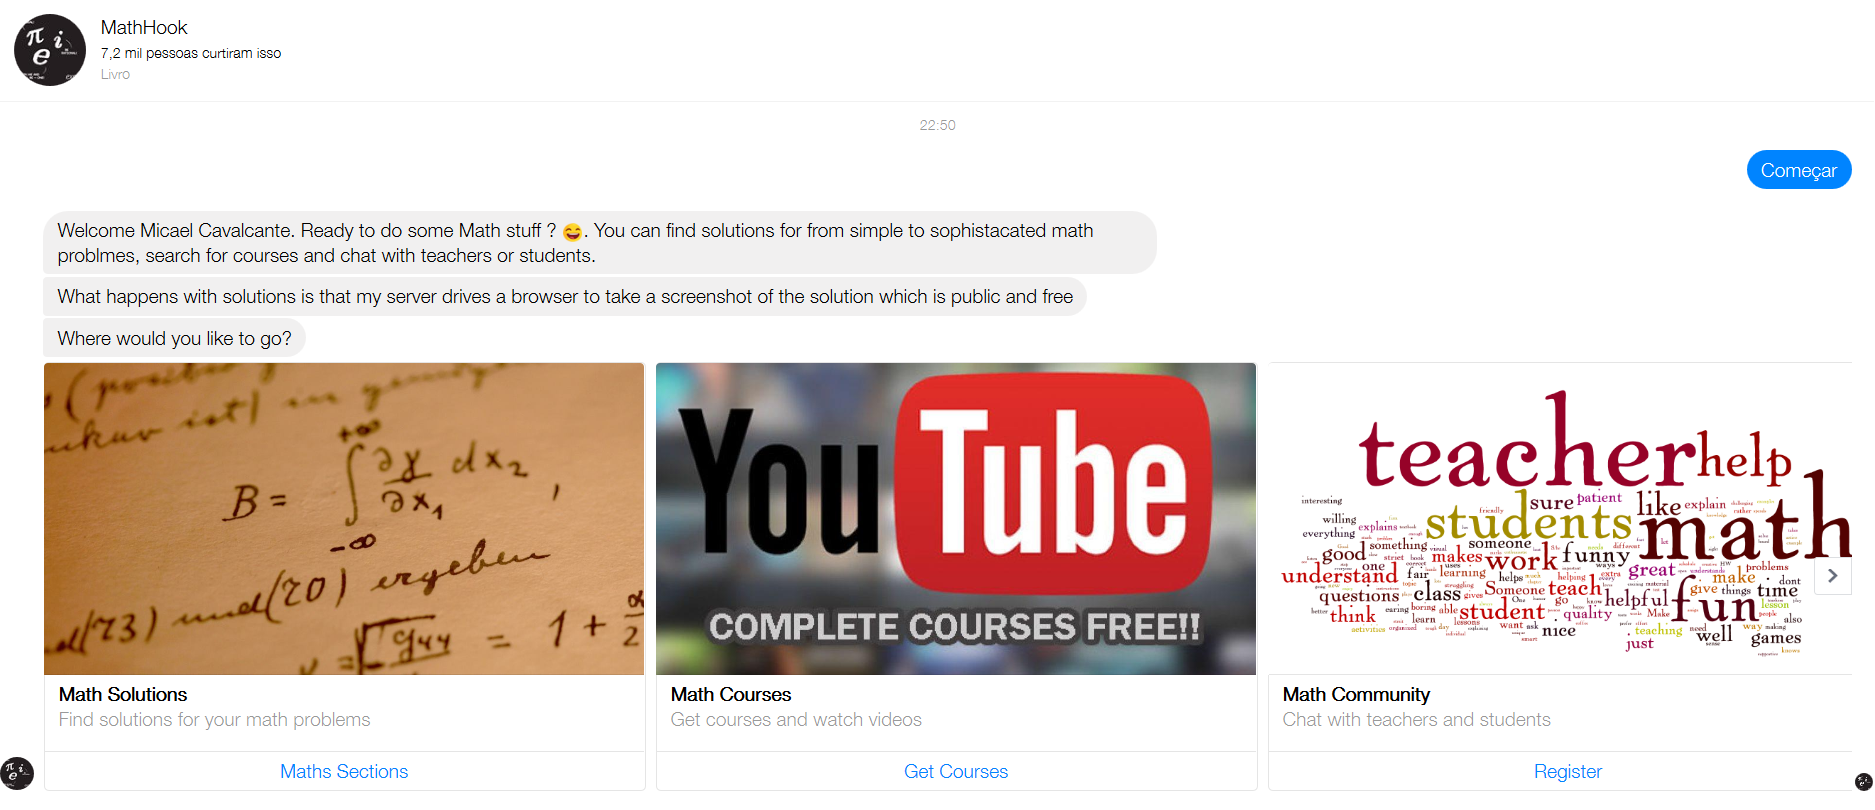
\includegraphics[width=1\linewidth]{img/bot1_1.png}
    \caption{Screenshot do primeiro contato com o MathHook bot.}
    \label{fig:bot1_1}
\end{figure}

Para prosseguir, escolhi o ramo ``Math Solutions'' a fim de encontrar soluções para alguns problemas matemáticos.
Para tal, bastou selecionar a opção ``Maths Sections''. Como resposta, o bot aguarda novamente uma escolha do usuário. Agora o aspecto é o ramo da aritmética.
\begin{figure}[h!tbp]
    \centering
    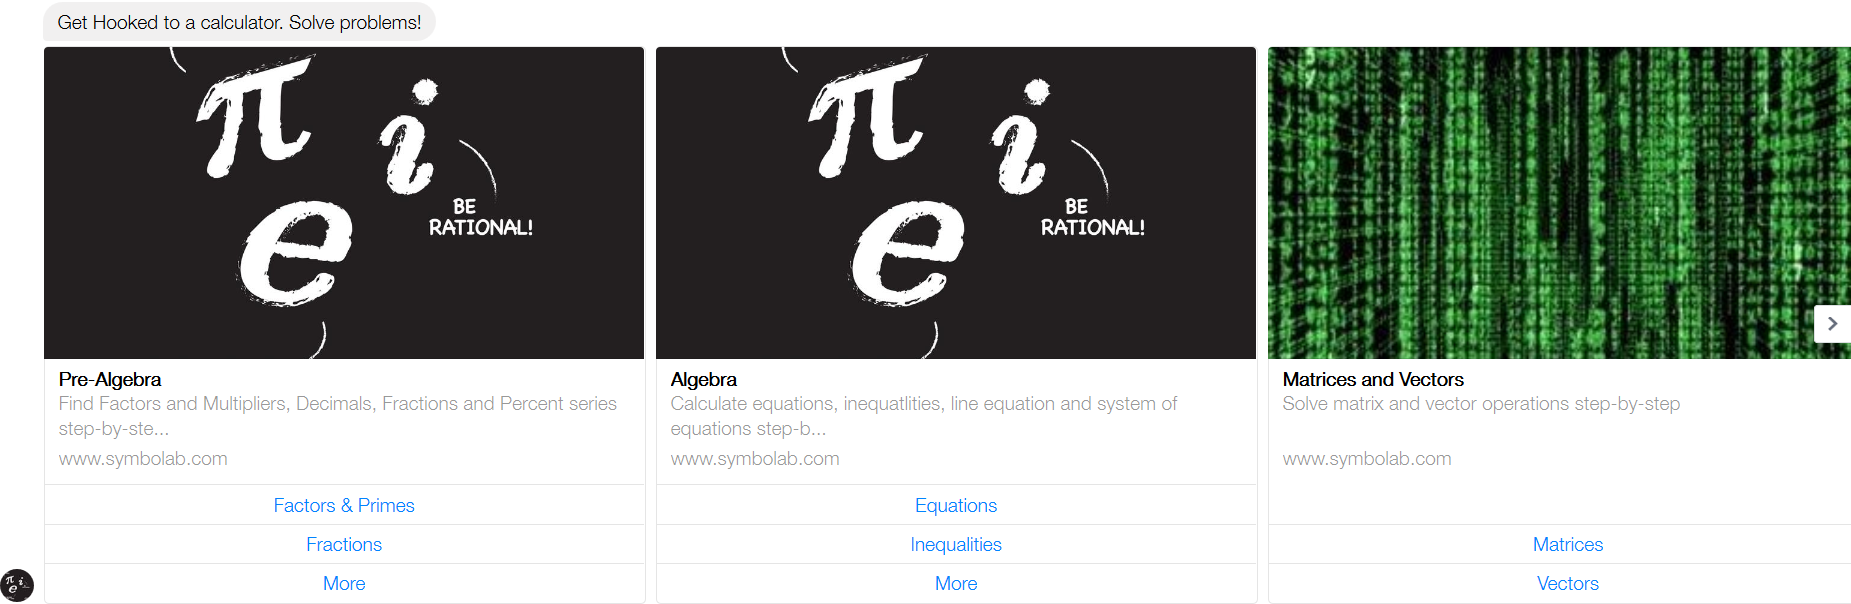
\includegraphics[width=0.65\linewidth]{img/bot1_2.png}
    \caption{Screenshot da resposta do MathHook ao escolher ``Maths Sections''.}
    \label{fig:bot1_2}
\end{figure}
O sistema suporta: pré-álgebra, álgebra, matrizes e vetores, funções e gráficos, trigonometria, pré-cálculo, cálculo e estatística (figura~\ref{fig:bot1_2}). 

Ao selecionar ``Equations'' (da categoria ``Pre Calculus''), o bot espera que o usuário faça outra escolha. Agora é sobre o método de equações que ele deseja calcular, podendo escolher entre 8 métodos, tais como: linear, quadrática, logarítmica, etc (figura~\ref{fig:bot1_3}).
\begin{figure}[h!tbp]
    \centering
    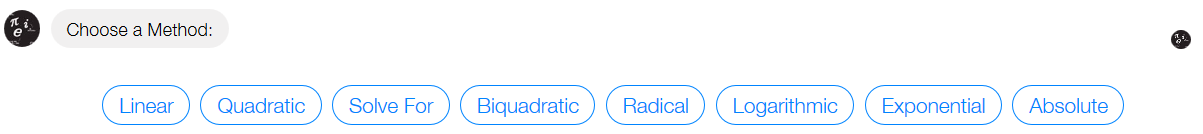
\includegraphics[width=1\linewidth]{img/bot1_3.png}
    \caption{Screenshot da resposta do MathHook ao escolher ``Equations''.}
    \label{fig:bot1_3}
\end{figure}

Vale ressaltar que durante a conversa, ao digitar uma mensagem que o bot não entende ou enviar uma mensagem quando o bot está esperando a escolha através de um clique em uma das opções, o mesmo responde com a seguinte mensagem interativa (pode ser vista na fig.~\ref{fig:bot1_4}):
\begin{description}
% \item \eu{Foo}
    \item \chatbot{I don't understand what you want try in another form :( Speciy What you meant}
    \item \chatbot{Speciy What you meant}
\end{description}

\begin{figure}[h!tbp]
    \centering
    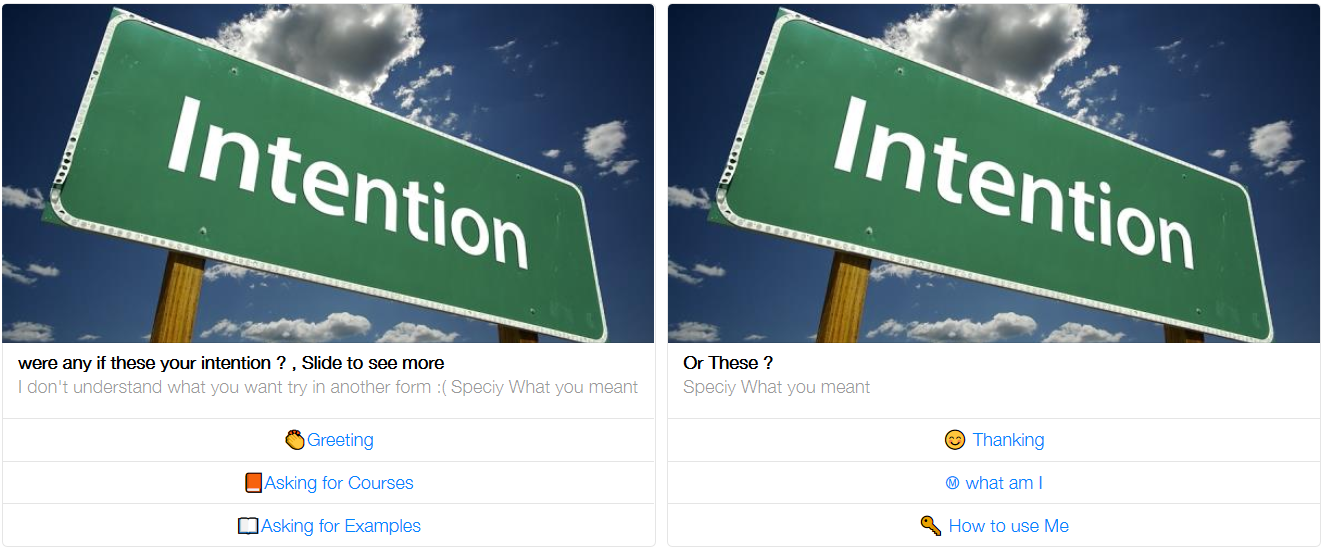
\includegraphics[width=1.1\linewidth]{img/bot1_4.png}
    \caption{Screenshot da resposta do MathHook para mensagens que ele não entende.}
    \label{fig:bot1_4}
\end{figure}

Continuando a conversação, escolhi o método (equação) Linear, assim, o bot responde (sobrescrevendo a mensagem de escolha dos métodos) com a mensagem abaixo e as opções ``Examples/Exercises'' e ``Detach'' (para interromper):
\begin{description}
    \item \chatbot{Now you're Linked to linear equation calculator. type your problem whenever you want to get examples press the button. Or type examples or detach whenever you want.}
\end{description}
Assim, espera que o usuário envie uma equação linear para ele resolver. Porém, ao escolher se desconectar, o bot continua solucionando os problemas. Além disso, ele também resolve qualquer problema, não estando diretamente relacionado ao método escolhido previamente.

Como meu objetivo é verificar (e validar) a solução encontrada para algum problema, a conversa se seguiu da seguinte forma:
\subsection{ChatterBot MathHook}\label{subsec:bot1}
\begin{figure}[h!tbp]
    \centering
    
\includegraphics[width=0.4\linewidth]{img/bot1_logo.png}
    \caption{Avatar do perfil do MathHook bot.}
    \label{fig:bot1_logo}
\end{figure}

Este foi desenvolvido para o aplicativo Messenger do Facebook, assim, pode ser acessado tanto por dispositivos móveis quanto computadores de mesa, desde que tenham o aplicativo instalado. Está atualmente na versão $1.2$ e possui o código aberto, disponível em \url{https://github.com/AhmedMashour/mHookBot}.
Para iniciar uma conversa com ele, basta ir ao seu site \url{http://mathhook.herokuapp.com} ou, encontrá-lo diretamente no aplicativo procurando por ``mathhook''.
Uma pequena demonstração do bot está disponível em vídeo publicado no YouTube no dia 31 de maio de 2017: \url{https://www.youtube.com/watch?v=4f_cMU70TmM}
Esse bot tem como objetivo tanto solucionar problemas matemáticos (soluções bem detalhadas) quanto entregar ao usuário informações que o ajudarão a aprender sobre algo do universo da matemática, oferecendo links de vídeo-aulas e o apoio da comunidade que o compõem.
A linguagem de programação utilizada foi o JavaScript e a língua que o sistema compreende e responde é o Inglês.

A interação com esse chatterbot é unidirecional e se inicia com qualquer mensagem do usuário enviando para ele.
O mesmo responde com mensagens de apresentação (vide a figura~\ref{fig:bot1_1}) e espera que o usuário escolha o que deseja que o bot lhe introduza, que pode ser: soluções, cursos ou acessar a comunidade.
\begin{figure}[h!tbp]
    \centering
    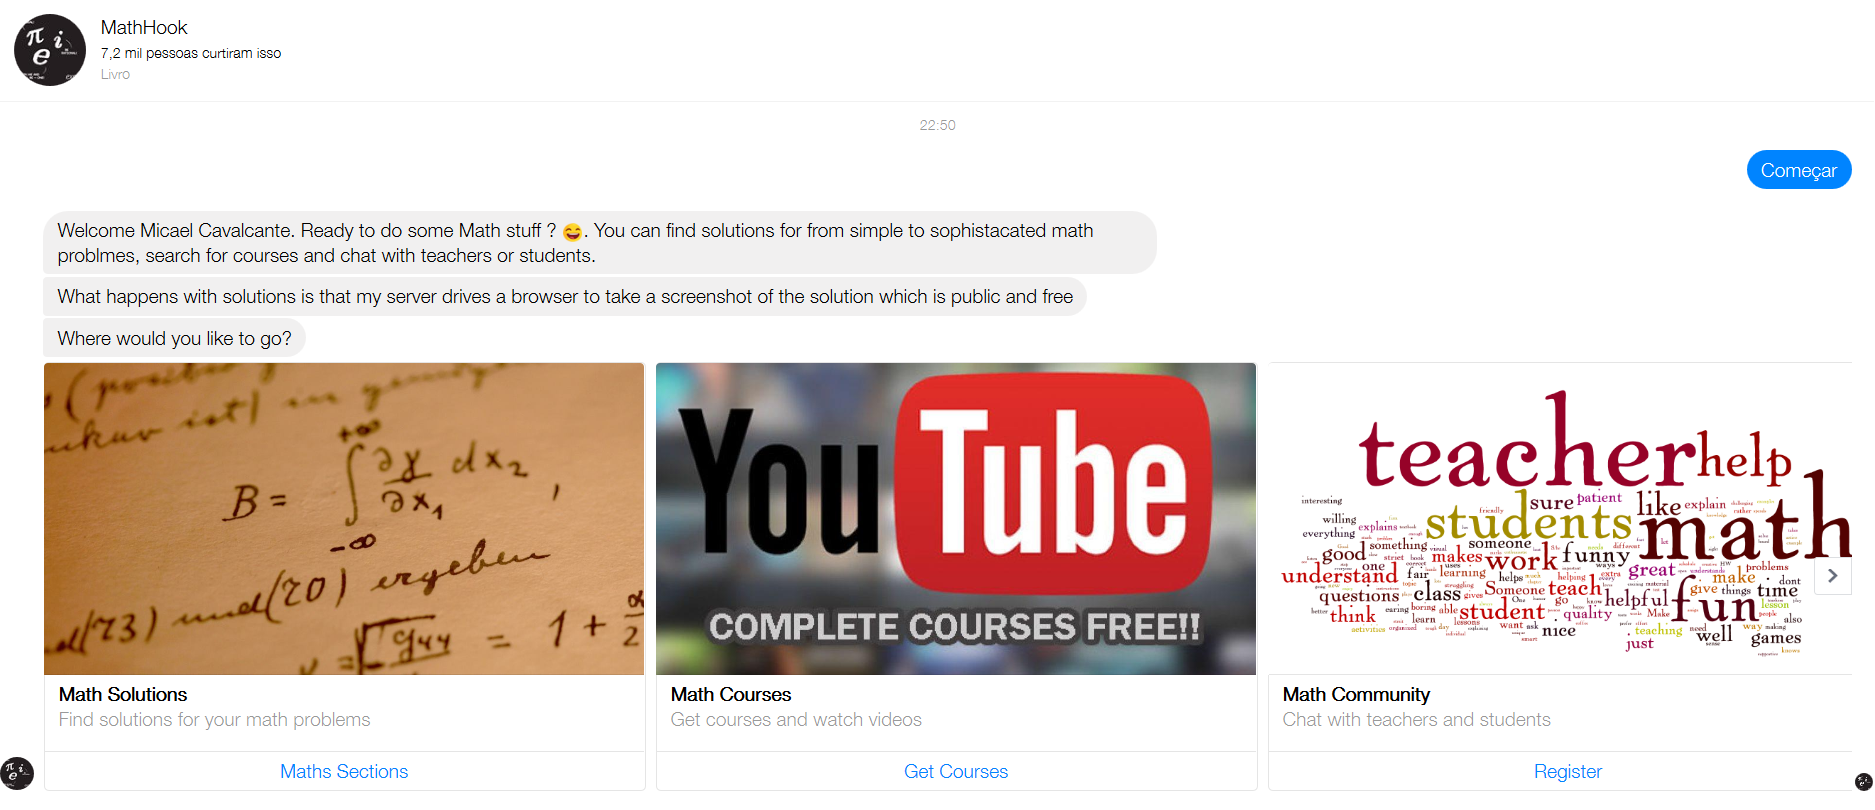
\includegraphics[width=1\linewidth]{img/bot1_1.png}
    \caption{Screenshot do primeiro contato com o MathHook bot.}
    \label{fig:bot1_1}
\end{figure}

Para prosseguir, escolhi o ramo ``Math Solutions'' a fim de encontrar soluções para alguns problemas matemáticos.
Para tal, bastou selecionar a opção ``Maths Sections''. Como resposta, o bot aguarda novamente uma escolha do usuário. Agora o aspecto é o ramo da aritmética.
\begin{figure}[h!tbp]
    \centering
    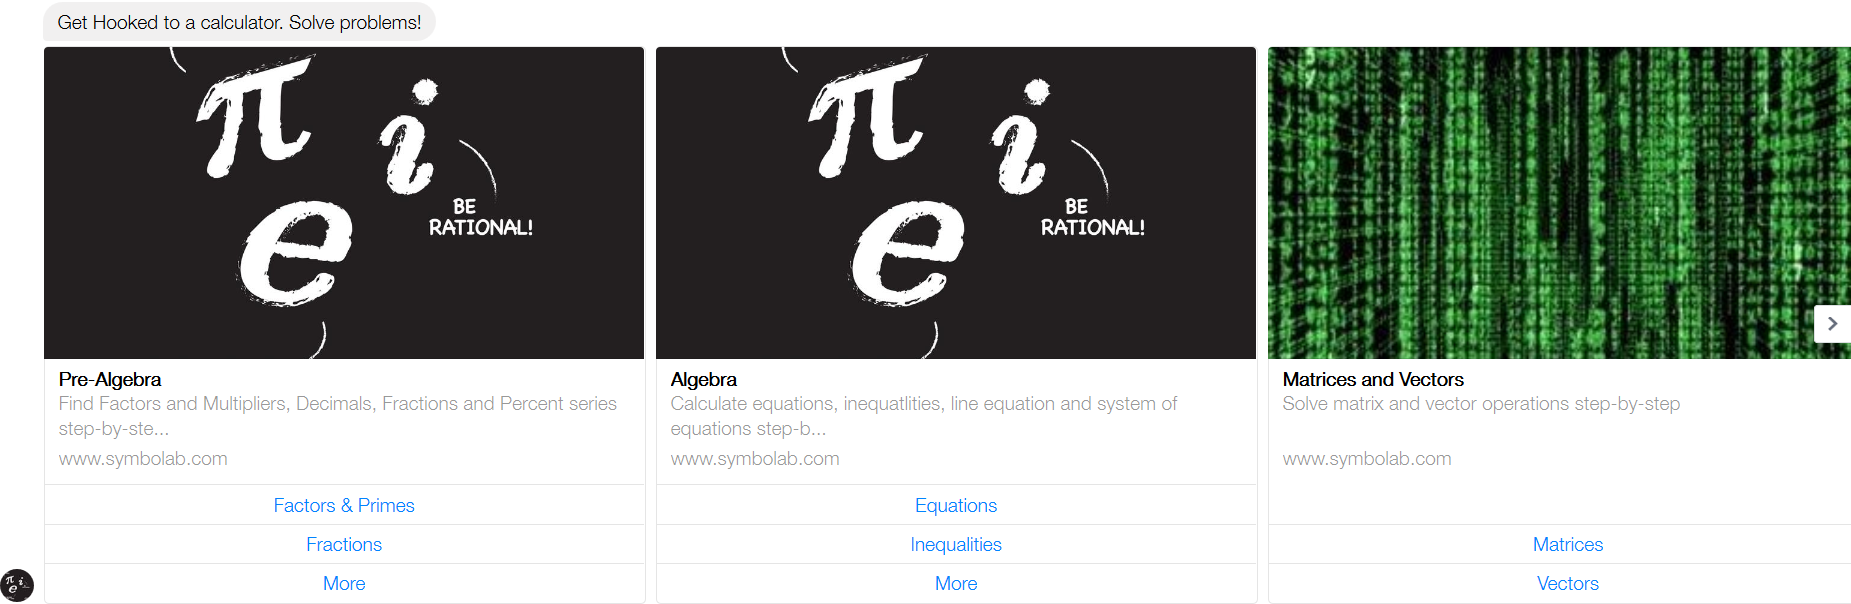
\includegraphics[width=0.65\linewidth]{img/bot1_2.png}
    \caption{Screenshot da resposta do MathHook ao escolher ``Maths Sections''.}
    \label{fig:bot1_2}
\end{figure}
O sistema suporta: pré-álgebra, álgebra, matrizes e vetores, funções e gráficos, trigonometria, pré-cálculo, cálculo e estatística (figura~\ref{fig:bot1_2}). 

Ao selecionar ``Equations'' (da categoria ``Pre Calculus''), o bot espera que o usuário faça outra escolha. Agora é sobre o método de equações que ele deseja calcular, podendo escolher entre 8 métodos, tais como: linear, quadrática, logarítmica, etc (figura~\ref{fig:bot1_3}).
\begin{figure}[h!tbp]
    \centering
    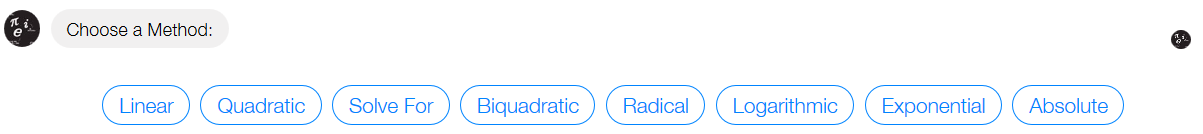
\includegraphics[width=1\linewidth]{img/bot1_3.png}
    \caption{Screenshot da resposta do MathHook ao escolher ``Equations''.}
    \label{fig:bot1_3}
\end{figure}

Vale ressaltar que durante a conversa, ao digitar uma mensagem que o bot não entende ou enviar uma mensagem quando o bot está esperando a escolha através de um clique em uma das opções, o mesmo responde com a seguinte mensagem interativa (pode ser vista na fig.~\ref{fig:bot1_4}):
\begin{description}
% \item \eu{Foo}
    \item \chatbot{I don't understand what you want try in another form :( Speciy What you meant}
    \item \chatbot{Speciy What you meant}
\end{description}

\begin{figure}[h!tbp]
    \centering
    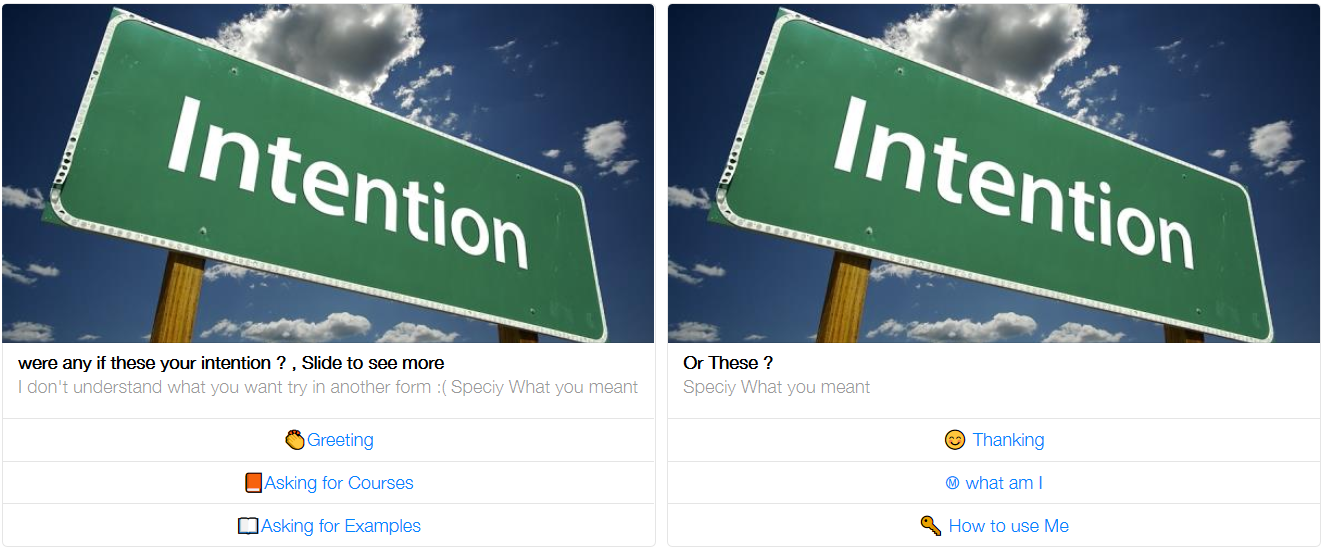
\includegraphics[width=1.1\linewidth]{img/bot1_4.png}
    \caption{Screenshot da resposta do MathHook para mensagens que ele não entende.}
    \label{fig:bot1_4}
\end{figure}

Continuando a conversação, escolhi o método (equação) Linear, assim, o bot responde (sobrescrevendo a mensagem de escolha dos métodos) com a mensagem abaixo e as opções ``Examples/Exercises'' e ``Detach'' (para interromper):
\begin{description}
    \item \chatbot{Now you're Linked to linear equation calculator. type your problem whenever you want to get examples press the button. Or type examples or detach whenever you want.}
\end{description}
Assim, espera que o usuário envie uma equação linear para ele resolver. Porém, ao escolher se desconectar, o bot continua solucionando os problemas. Além disso, ele também resolve qualquer problema, não estando diretamente relacionado ao método escolhido previamente.

Como meu objetivo é verificar (e validar) a solução encontrada para algum problema, a conversa se seguiu da seguinte forma:
\subsection{ChatterBot MathHook}\label{subsec:bot1}
\begin{figure}[h!tbp]
    \centering
    
\includegraphics[width=0.4\linewidth]{img/bot1_logo.png}
    \caption{Avatar do perfil do MathHook bot.}
    \label{fig:bot1_logo}
\end{figure}

Este foi desenvolvido para o aplicativo Messenger do Facebook, assim, pode ser acessado tanto por dispositivos móveis quanto computadores de mesa, desde que tenham o aplicativo instalado. Está atualmente na versão $1.2$ e possui o código aberto, disponível em \url{https://github.com/AhmedMashour/mHookBot}.
Para iniciar uma conversa com ele, basta ir ao seu site \url{http://mathhook.herokuapp.com} ou, encontrá-lo diretamente no aplicativo procurando por ``mathhook''.
Uma pequena demonstração do bot está disponível em vídeo publicado no YouTube no dia 31 de maio de 2017: \url{https://www.youtube.com/watch?v=4f_cMU70TmM}
Esse bot tem como objetivo tanto solucionar problemas matemáticos (soluções bem detalhadas) quanto entregar ao usuário informações que o ajudarão a aprender sobre algo do universo da matemática, oferecendo links de vídeo-aulas e o apoio da comunidade que o compõem.
A linguagem de programação utilizada foi o JavaScript e a língua que o sistema compreende e responde é o Inglês.

A interação com esse chatterbot é unidirecional e se inicia com qualquer mensagem do usuário enviando para ele.
O mesmo responde com mensagens de apresentação (vide a figura~\ref{fig:bot1_1}) e espera que o usuário escolha o que deseja que o bot lhe introduza, que pode ser: soluções, cursos ou acessar a comunidade.
\begin{figure}[h!tbp]
    \centering
    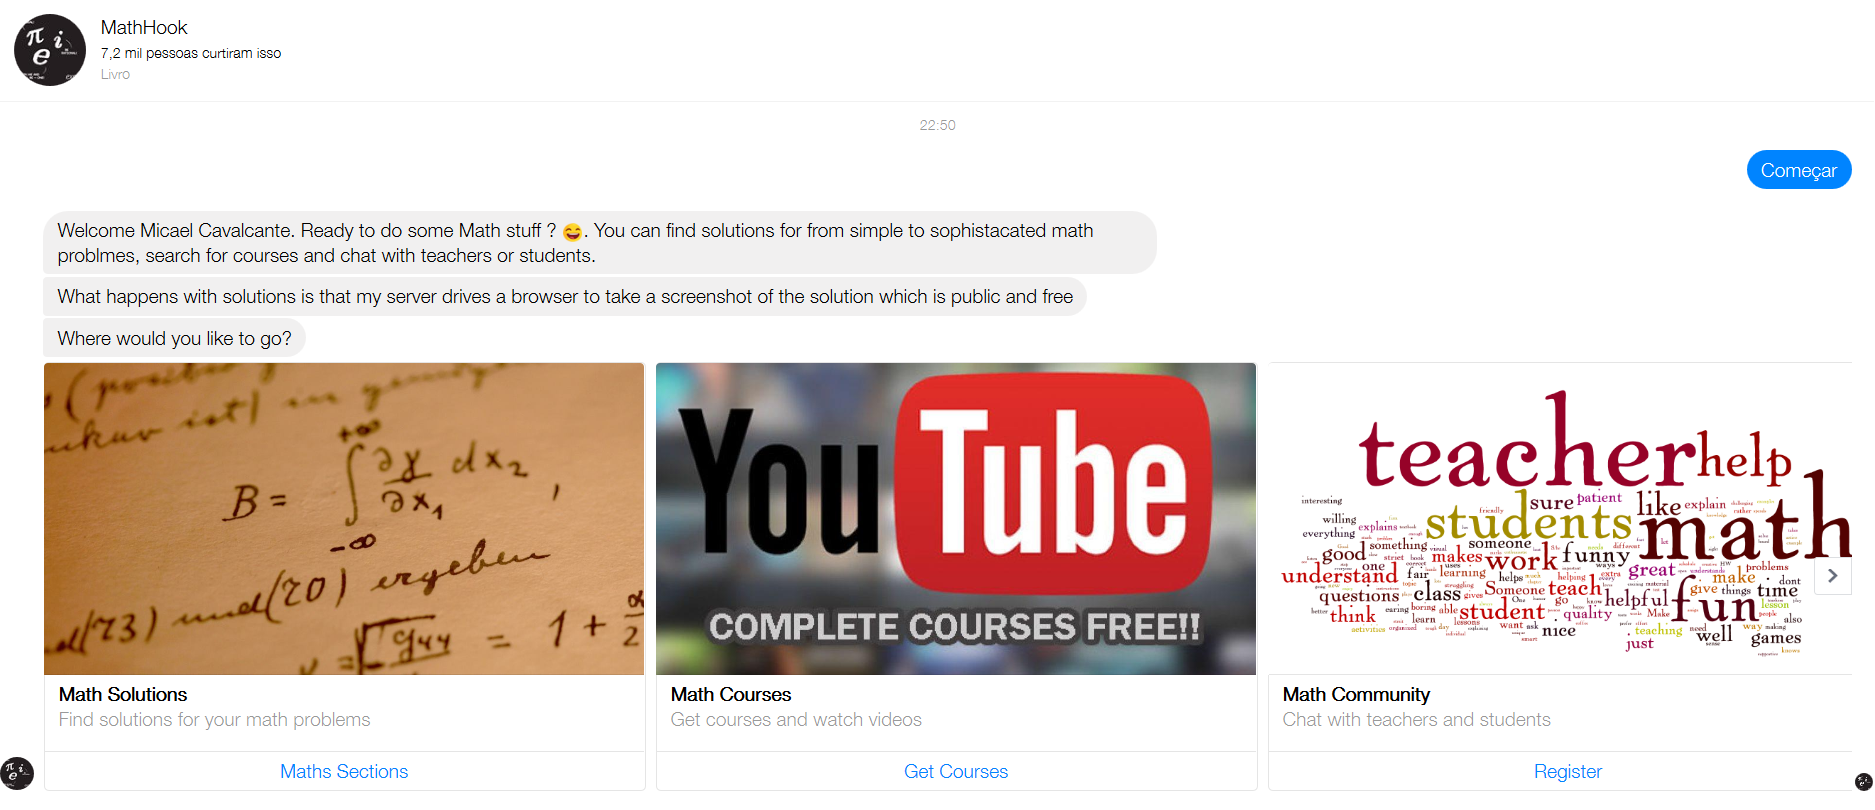
\includegraphics[width=1\linewidth]{img/bot1_1.png}
    \caption{Screenshot do primeiro contato com o MathHook bot.}
    \label{fig:bot1_1}
\end{figure}

Para prosseguir, escolhi o ramo ``Math Solutions'' a fim de encontrar soluções para alguns problemas matemáticos.
Para tal, bastou selecionar a opção ``Maths Sections''. Como resposta, o bot aguarda novamente uma escolha do usuário. Agora o aspecto é o ramo da aritmética.
\begin{figure}[h!tbp]
    \centering
    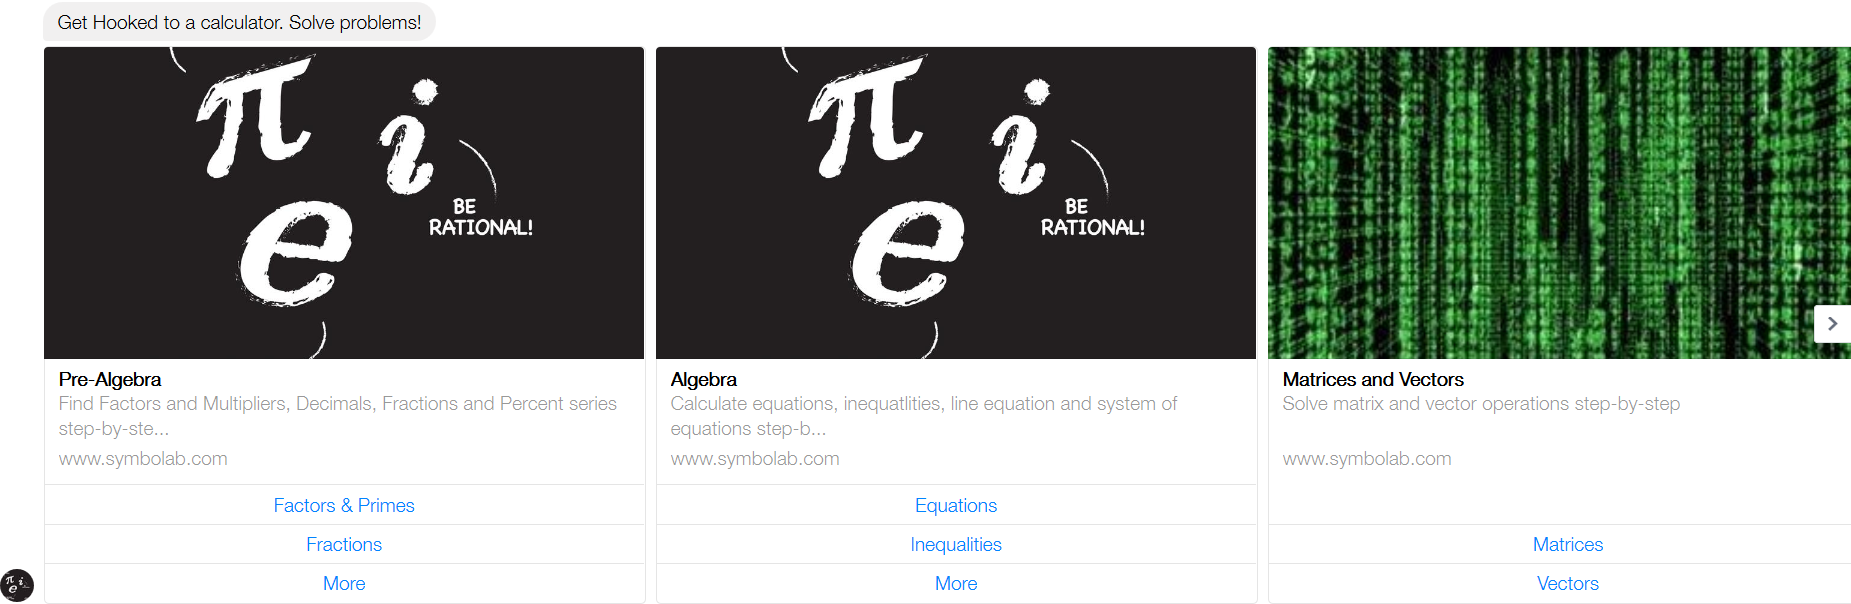
\includegraphics[width=0.65\linewidth]{img/bot1_2.png}
    \caption{Screenshot da resposta do MathHook ao escolher ``Maths Sections''.}
    \label{fig:bot1_2}
\end{figure}
O sistema suporta: pré-álgebra, álgebra, matrizes e vetores, funções e gráficos, trigonometria, pré-cálculo, cálculo e estatística (figura~\ref{fig:bot1_2}). 

Ao selecionar ``Equations'' (da categoria ``Pre Calculus''), o bot espera que o usuário faça outra escolha. Agora é sobre o método de equações que ele deseja calcular, podendo escolher entre 8 métodos, tais como: linear, quadrática, logarítmica, etc (figura~\ref{fig:bot1_3}).
\begin{figure}[h!tbp]
    \centering
    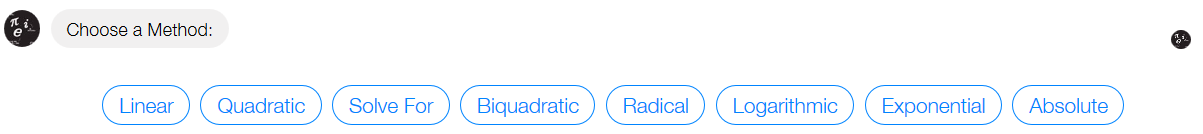
\includegraphics[width=1\linewidth]{img/bot1_3.png}
    \caption{Screenshot da resposta do MathHook ao escolher ``Equations''.}
    \label{fig:bot1_3}
\end{figure}

Vale ressaltar que durante a conversa, ao digitar uma mensagem que o bot não entende ou enviar uma mensagem quando o bot está esperando a escolha através de um clique em uma das opções, o mesmo responde com a seguinte mensagem interativa (pode ser vista na fig.~\ref{fig:bot1_4}):
\begin{description}
% \item \eu{Foo}
    \item \chatbot{I don't understand what you want try in another form :( Speciy What you meant}
    \item \chatbot{Speciy What you meant}
\end{description}

\begin{figure}[h!tbp]
    \centering
    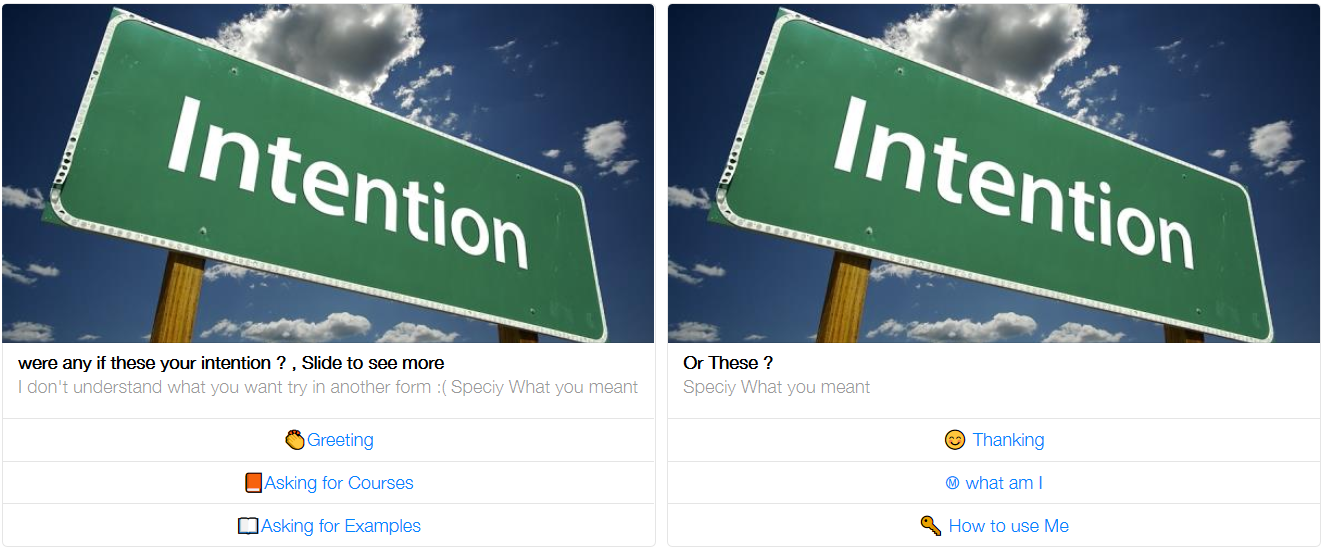
\includegraphics[width=1.1\linewidth]{img/bot1_4.png}
    \caption{Screenshot da resposta do MathHook para mensagens que ele não entende.}
    \label{fig:bot1_4}
\end{figure}

Continuando a conversação, escolhi o método (equação) Linear, assim, o bot responde (sobrescrevendo a mensagem de escolha dos métodos) com a mensagem abaixo e as opções ``Examples/Exercises'' e ``Detach'' (para interromper):
\begin{description}
    \item \chatbot{Now you're Linked to linear equation calculator. type your problem whenever you want to get examples press the button. Or type examples or detach whenever you want.}
\end{description}
Assim, espera que o usuário envie uma equação linear para ele resolver. Porém, ao escolher se desconectar, o bot continua solucionando os problemas. Além disso, ele também resolve qualquer problema, não estando diretamente relacionado ao método escolhido previamente.

Como meu objetivo é verificar (e validar) a solução encontrada para algum problema, a conversa se seguiu da seguinte forma:
\subsection{ChatterBot MathHook}\label{subsec:bot1}
\input{img/bot1_logo}

Este foi desenvolvido para o aplicativo Messenger do Facebook, assim, pode ser acessado tanto por dispositivos móveis quanto computadores de mesa, desde que tenham o aplicativo instalado. Está atualmente na versão $1.2$ e possui o código aberto, disponível em \url{https://github.com/AhmedMashour/mHookBot}.
Para iniciar uma conversa com ele, basta ir ao seu site \url{http://mathhook.herokuapp.com} ou, encontrá-lo diretamente no aplicativo procurando por ``mathhook''.
Uma pequena demonstração do bot está disponível em vídeo publicado no YouTube no dia 31 de maio de 2017: \url{https://www.youtube.com/watch?v=4f_cMU70TmM}
Esse bot tem como objetivo tanto solucionar problemas matemáticos (soluções bem detalhadas) quanto entregar ao usuário informações que o ajudarão a aprender sobre algo do universo da matemática, oferecendo links de vídeo-aulas e o apoio da comunidade que o compõem.
A linguagem de programação utilizada foi o JavaScript e a língua que o sistema compreende e responde é o Inglês.

A interação com esse chatterbot é unidirecional e se inicia com qualquer mensagem do usuário enviando para ele.
O mesmo responde com mensagens de apresentação (vide a figura~\ref{fig:bot1_1}) e espera que o usuário escolha o que deseja que o bot lhe introduza, que pode ser: soluções, cursos ou acessar a comunidade.
\input{img/bot1_1}

Para prosseguir, escolhi o ramo ``Math Solutions'' a fim de encontrar soluções para alguns problemas matemáticos.
Para tal, bastou selecionar a opção ``Maths Sections''. Como resposta, o bot aguarda novamente uma escolha do usuário. Agora o aspecto é o ramo da aritmética.
\input{img/bot1_2}
O sistema suporta: pré-álgebra, álgebra, matrizes e vetores, funções e gráficos, trigonometria, pré-cálculo, cálculo e estatística (figura~\ref{fig:bot1_2}). 

Ao selecionar ``Equations'' (da categoria ``Pre Calculus''), o bot espera que o usuário faça outra escolha. Agora é sobre o método de equações que ele deseja calcular, podendo escolher entre 8 métodos, tais como: linear, quadrática, logarítmica, etc (figura~\ref{fig:bot1_3}).
\input{img/bot1_3}

Vale ressaltar que durante a conversa, ao digitar uma mensagem que o bot não entende ou enviar uma mensagem quando o bot está esperando a escolha através de um clique em uma das opções, o mesmo responde com a seguinte mensagem interativa (pode ser vista na fig.~\ref{fig:bot1_4}):
\begin{description}
% \item \eu{Foo}
    \item \chatbot{I don't understand what you want try in another form :( Speciy What you meant}
    \item \chatbot{Speciy What you meant}
\end{description}

\input{img/bot1_4}

Continuando a conversação, escolhi o método (equação) Linear, assim, o bot responde (sobrescrevendo a mensagem de escolha dos métodos) com a mensagem abaixo e as opções ``Examples/Exercises'' e ``Detach'' (para interromper):
\begin{description}
    \item \chatbot{Now you're Linked to linear equation calculator. type your problem whenever you want to get examples press the button. Or type examples or detach whenever you want.}
\end{description}
Assim, espera que o usuário envie uma equação linear para ele resolver. Porém, ao escolher se desconectar, o bot continua solucionando os problemas. Além disso, ele também resolve qualquer problema, não estando diretamente relacionado ao método escolhido previamente.

Como meu objetivo é verificar (e validar) a solução encontrada para algum problema, a conversa se seguiu da seguinte forma:
\input{conversas/bot1}
E uma imagem (em baixa qualidade) da solução \emph{correta} etapa-por-etapa da expressão, além das opções ``Press Here'' para verificar melhor a solução e o botão ``Compartilhar'' (fig.~\ref{fig:bot1_5}).
\input{img/bot1_5}

A tabela~\ref{tab:bot1} abaixo lista as vantagens e desvantagens que encontrei após um período de conversação com esse chatterbot.
\input{tables/bot1}

Segue uma lista de melhorias e correções que eu sugiro ao sistema:
\begin{itemize}[noitemsep]
    \item Adicionar uma mensagem de ajuda padrão (e.g., ``help'')
    \item Reduzir o fluxo para os principais objetivos
    \item Permitir que o usuário digite uma das opções e envie como mensagem
    \item Corrigir identificação de expressões em textos (prever erros do usuário)
    \item Detalhar opções que o usuário possui
\end{itemize}
E uma imagem (em baixa qualidade) da solução \emph{correta} etapa-por-etapa da expressão, além das opções ``Press Here'' para verificar melhor a solução e o botão ``Compartilhar'' (fig.~\ref{fig:bot1_5}).
\begin{figure}[h!tbp]
    \centering
    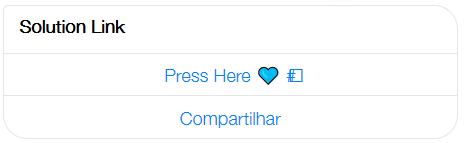
\includegraphics[width=0.7\linewidth]{img/bot1_5.png}
    \caption{Screenshot das opções exibidas pelo MathHook após solucionar um problema matemático.}
    \label{fig:bot1_5}
\end{figure}

A tabela~\ref{tab:bot1} abaixo lista as vantagens e desvantagens que encontrei após um período de conversação com esse chatterbot.
\subsection{ChatterBot MathHook}\label{subsec:bot1}
\input{img/bot1_logo}

Este foi desenvolvido para o aplicativo Messenger do Facebook, assim, pode ser acessado tanto por dispositivos móveis quanto computadores de mesa, desde que tenham o aplicativo instalado. Está atualmente na versão $1.2$ e possui o código aberto, disponível em \url{https://github.com/AhmedMashour/mHookBot}.
Para iniciar uma conversa com ele, basta ir ao seu site \url{http://mathhook.herokuapp.com} ou, encontrá-lo diretamente no aplicativo procurando por ``mathhook''.
Uma pequena demonstração do bot está disponível em vídeo publicado no YouTube no dia 31 de maio de 2017: \url{https://www.youtube.com/watch?v=4f_cMU70TmM}
Esse bot tem como objetivo tanto solucionar problemas matemáticos (soluções bem detalhadas) quanto entregar ao usuário informações que o ajudarão a aprender sobre algo do universo da matemática, oferecendo links de vídeo-aulas e o apoio da comunidade que o compõem.
A linguagem de programação utilizada foi o JavaScript e a língua que o sistema compreende e responde é o Inglês.

A interação com esse chatterbot é unidirecional e se inicia com qualquer mensagem do usuário enviando para ele.
O mesmo responde com mensagens de apresentação (vide a figura~\ref{fig:bot1_1}) e espera que o usuário escolha o que deseja que o bot lhe introduza, que pode ser: soluções, cursos ou acessar a comunidade.
\input{img/bot1_1}

Para prosseguir, escolhi o ramo ``Math Solutions'' a fim de encontrar soluções para alguns problemas matemáticos.
Para tal, bastou selecionar a opção ``Maths Sections''. Como resposta, o bot aguarda novamente uma escolha do usuário. Agora o aspecto é o ramo da aritmética.
\input{img/bot1_2}
O sistema suporta: pré-álgebra, álgebra, matrizes e vetores, funções e gráficos, trigonometria, pré-cálculo, cálculo e estatística (figura~\ref{fig:bot1_2}). 

Ao selecionar ``Equations'' (da categoria ``Pre Calculus''), o bot espera que o usuário faça outra escolha. Agora é sobre o método de equações que ele deseja calcular, podendo escolher entre 8 métodos, tais como: linear, quadrática, logarítmica, etc (figura~\ref{fig:bot1_3}).
\input{img/bot1_3}

Vale ressaltar que durante a conversa, ao digitar uma mensagem que o bot não entende ou enviar uma mensagem quando o bot está esperando a escolha através de um clique em uma das opções, o mesmo responde com a seguinte mensagem interativa (pode ser vista na fig.~\ref{fig:bot1_4}):
\begin{description}
% \item \eu{Foo}
    \item \chatbot{I don't understand what you want try in another form :( Speciy What you meant}
    \item \chatbot{Speciy What you meant}
\end{description}

\input{img/bot1_4}

Continuando a conversação, escolhi o método (equação) Linear, assim, o bot responde (sobrescrevendo a mensagem de escolha dos métodos) com a mensagem abaixo e as opções ``Examples/Exercises'' e ``Detach'' (para interromper):
\begin{description}
    \item \chatbot{Now you're Linked to linear equation calculator. type your problem whenever you want to get examples press the button. Or type examples or detach whenever you want.}
\end{description}
Assim, espera que o usuário envie uma equação linear para ele resolver. Porém, ao escolher se desconectar, o bot continua solucionando os problemas. Além disso, ele também resolve qualquer problema, não estando diretamente relacionado ao método escolhido previamente.

Como meu objetivo é verificar (e validar) a solução encontrada para algum problema, a conversa se seguiu da seguinte forma:
\input{conversas/bot1}
E uma imagem (em baixa qualidade) da solução \emph{correta} etapa-por-etapa da expressão, além das opções ``Press Here'' para verificar melhor a solução e o botão ``Compartilhar'' (fig.~\ref{fig:bot1_5}).
\input{img/bot1_5}

A tabela~\ref{tab:bot1} abaixo lista as vantagens e desvantagens que encontrei após um período de conversação com esse chatterbot.
\input{tables/bot1}

Segue uma lista de melhorias e correções que eu sugiro ao sistema:
\begin{itemize}[noitemsep]
    \item Adicionar uma mensagem de ajuda padrão (e.g., ``help'')
    \item Reduzir o fluxo para os principais objetivos
    \item Permitir que o usuário digite uma das opções e envie como mensagem
    \item Corrigir identificação de expressões em textos (prever erros do usuário)
    \item Detalhar opções que o usuário possui
\end{itemize}

Segue uma lista de melhorias e correções que eu sugiro ao sistema:
\begin{itemize}[noitemsep]
    \item Adicionar uma mensagem de ajuda padrão (e.g., ``help'')
    \item Reduzir o fluxo para os principais objetivos
    \item Permitir que o usuário digite uma das opções e envie como mensagem
    \item Corrigir identificação de expressões em textos (prever erros do usuário)
    \item Detalhar opções que o usuário possui
\end{itemize}
E uma imagem (em baixa qualidade) da solução \emph{correta} etapa-por-etapa da expressão, além das opções ``Press Here'' para verificar melhor a solução e o botão ``Compartilhar'' (fig.~\ref{fig:bot1_5}).
\begin{figure}[h!tbp]
    \centering
    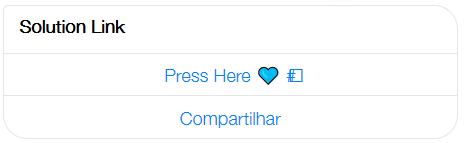
\includegraphics[width=0.7\linewidth]{img/bot1_5.png}
    \caption{Screenshot das opções exibidas pelo MathHook após solucionar um problema matemático.}
    \label{fig:bot1_5}
\end{figure}

A tabela~\ref{tab:bot1} abaixo lista as vantagens e desvantagens que encontrei após um período de conversação com esse chatterbot.
\subsection{ChatterBot MathHook}\label{subsec:bot1}
\begin{figure}[h!tbp]
    \centering
    
\includegraphics[width=0.4\linewidth]{img/bot1_logo.png}
    \caption{Avatar do perfil do MathHook bot.}
    \label{fig:bot1_logo}
\end{figure}

Este foi desenvolvido para o aplicativo Messenger do Facebook, assim, pode ser acessado tanto por dispositivos móveis quanto computadores de mesa, desde que tenham o aplicativo instalado. Está atualmente na versão $1.2$ e possui o código aberto, disponível em \url{https://github.com/AhmedMashour/mHookBot}.
Para iniciar uma conversa com ele, basta ir ao seu site \url{http://mathhook.herokuapp.com} ou, encontrá-lo diretamente no aplicativo procurando por ``mathhook''.
Uma pequena demonstração do bot está disponível em vídeo publicado no YouTube no dia 31 de maio de 2017: \url{https://www.youtube.com/watch?v=4f_cMU70TmM}
Esse bot tem como objetivo tanto solucionar problemas matemáticos (soluções bem detalhadas) quanto entregar ao usuário informações que o ajudarão a aprender sobre algo do universo da matemática, oferecendo links de vídeo-aulas e o apoio da comunidade que o compõem.
A linguagem de programação utilizada foi o JavaScript e a língua que o sistema compreende e responde é o Inglês.

A interação com esse chatterbot é unidirecional e se inicia com qualquer mensagem do usuário enviando para ele.
O mesmo responde com mensagens de apresentação (vide a figura~\ref{fig:bot1_1}) e espera que o usuário escolha o que deseja que o bot lhe introduza, que pode ser: soluções, cursos ou acessar a comunidade.
\begin{figure}[h!tbp]
    \centering
    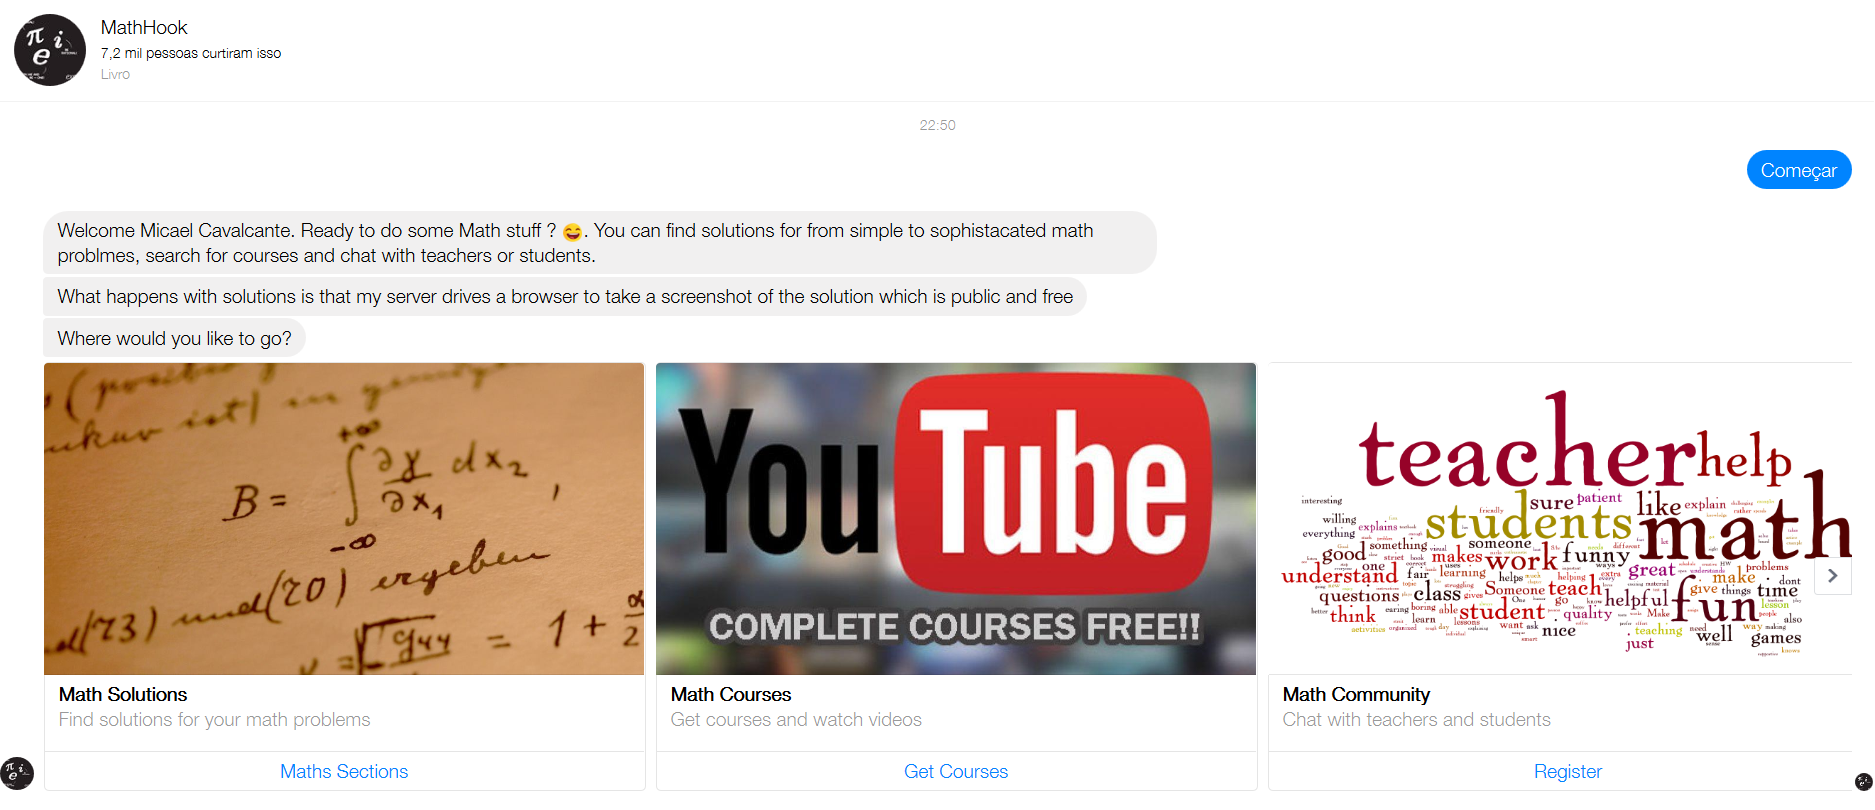
\includegraphics[width=1\linewidth]{img/bot1_1.png}
    \caption{Screenshot do primeiro contato com o MathHook bot.}
    \label{fig:bot1_1}
\end{figure}

Para prosseguir, escolhi o ramo ``Math Solutions'' a fim de encontrar soluções para alguns problemas matemáticos.
Para tal, bastou selecionar a opção ``Maths Sections''. Como resposta, o bot aguarda novamente uma escolha do usuário. Agora o aspecto é o ramo da aritmética.
\begin{figure}[h!tbp]
    \centering
    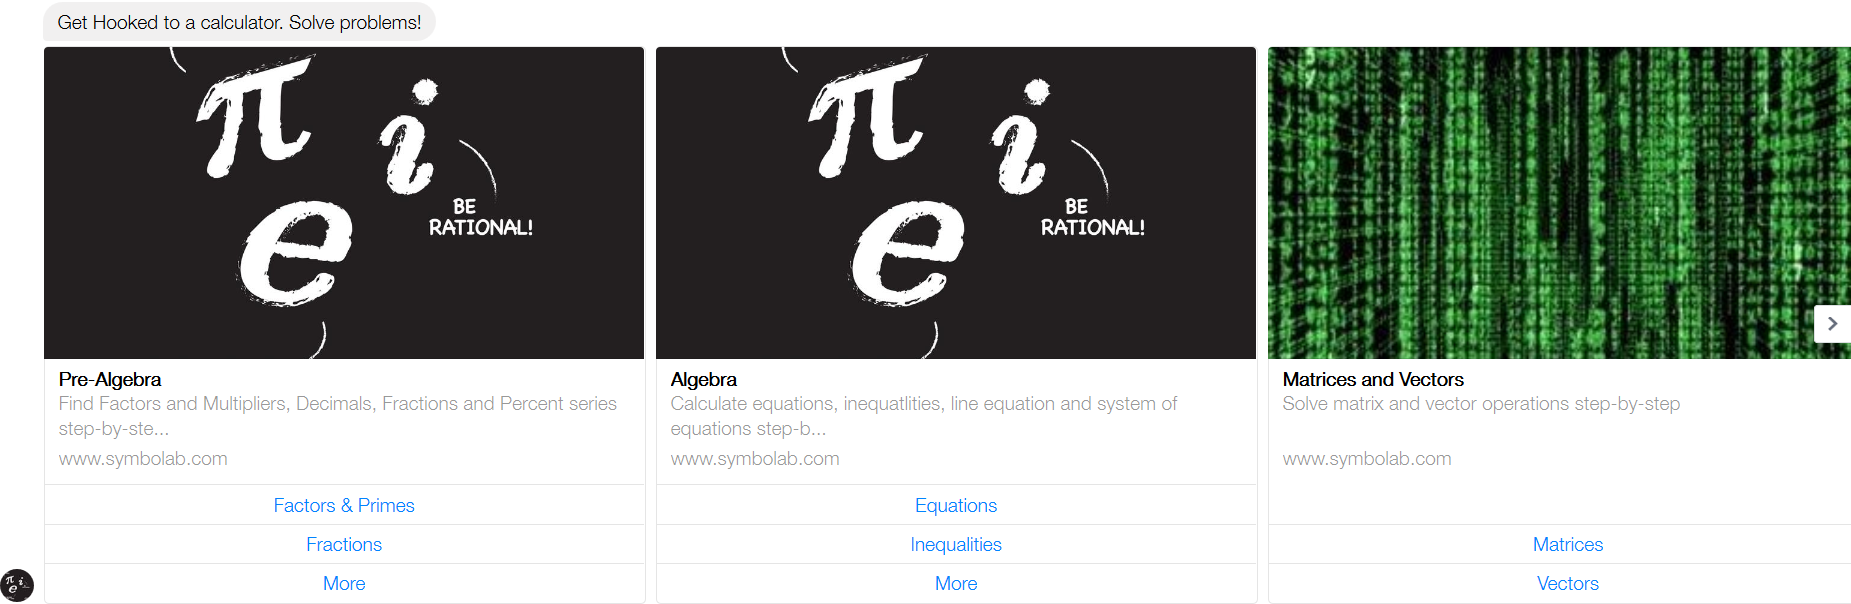
\includegraphics[width=0.65\linewidth]{img/bot1_2.png}
    \caption{Screenshot da resposta do MathHook ao escolher ``Maths Sections''.}
    \label{fig:bot1_2}
\end{figure}
O sistema suporta: pré-álgebra, álgebra, matrizes e vetores, funções e gráficos, trigonometria, pré-cálculo, cálculo e estatística (figura~\ref{fig:bot1_2}). 

Ao selecionar ``Equations'' (da categoria ``Pre Calculus''), o bot espera que o usuário faça outra escolha. Agora é sobre o método de equações que ele deseja calcular, podendo escolher entre 8 métodos, tais como: linear, quadrática, logarítmica, etc (figura~\ref{fig:bot1_3}).
\begin{figure}[h!tbp]
    \centering
    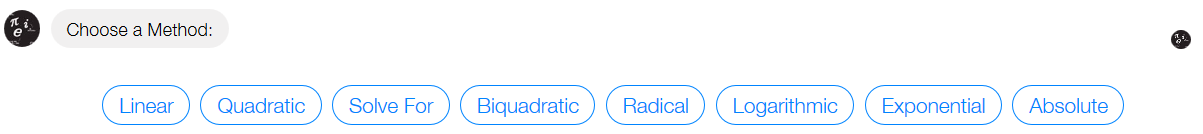
\includegraphics[width=1\linewidth]{img/bot1_3.png}
    \caption{Screenshot da resposta do MathHook ao escolher ``Equations''.}
    \label{fig:bot1_3}
\end{figure}

Vale ressaltar que durante a conversa, ao digitar uma mensagem que o bot não entende ou enviar uma mensagem quando o bot está esperando a escolha através de um clique em uma das opções, o mesmo responde com a seguinte mensagem interativa (pode ser vista na fig.~\ref{fig:bot1_4}):
\begin{description}
% \item \eu{Foo}
    \item \chatbot{I don't understand what you want try in another form :( Speciy What you meant}
    \item \chatbot{Speciy What you meant}
\end{description}

\begin{figure}[h!tbp]
    \centering
    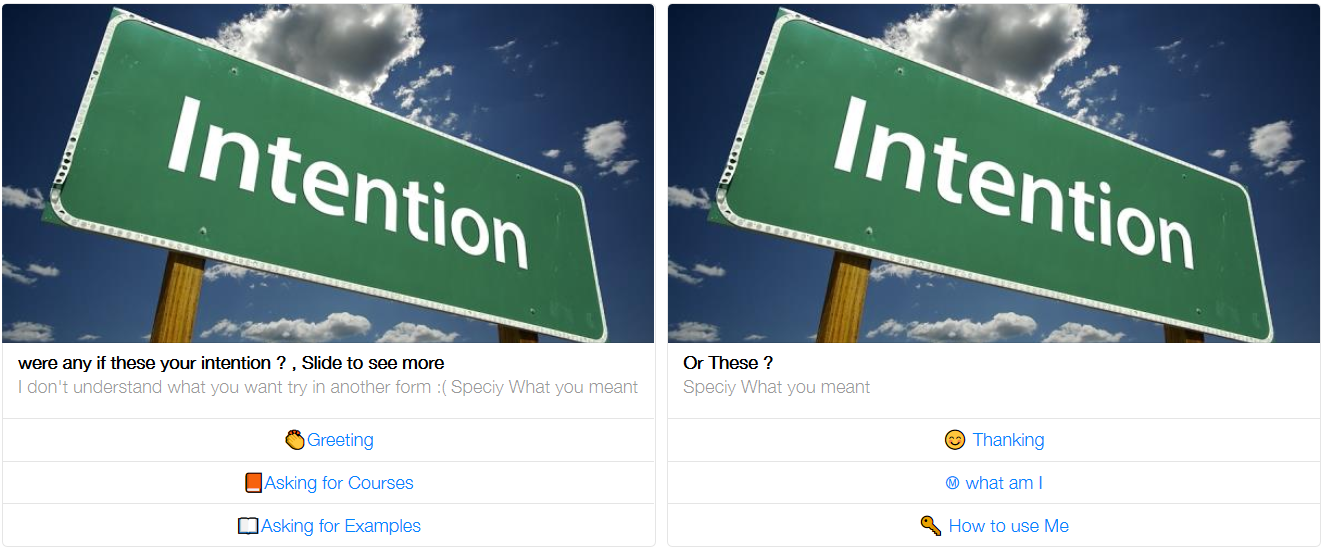
\includegraphics[width=1.1\linewidth]{img/bot1_4.png}
    \caption{Screenshot da resposta do MathHook para mensagens que ele não entende.}
    \label{fig:bot1_4}
\end{figure}

Continuando a conversação, escolhi o método (equação) Linear, assim, o bot responde (sobrescrevendo a mensagem de escolha dos métodos) com a mensagem abaixo e as opções ``Examples/Exercises'' e ``Detach'' (para interromper):
\begin{description}
    \item \chatbot{Now you're Linked to linear equation calculator. type your problem whenever you want to get examples press the button. Or type examples or detach whenever you want.}
\end{description}
Assim, espera que o usuário envie uma equação linear para ele resolver. Porém, ao escolher se desconectar, o bot continua solucionando os problemas. Além disso, ele também resolve qualquer problema, não estando diretamente relacionado ao método escolhido previamente.

Como meu objetivo é verificar (e validar) a solução encontrada para algum problema, a conversa se seguiu da seguinte forma:
\subsection{ChatterBot MathHook}\label{subsec:bot1}
\input{img/bot1_logo}

Este foi desenvolvido para o aplicativo Messenger do Facebook, assim, pode ser acessado tanto por dispositivos móveis quanto computadores de mesa, desde que tenham o aplicativo instalado. Está atualmente na versão $1.2$ e possui o código aberto, disponível em \url{https://github.com/AhmedMashour/mHookBot}.
Para iniciar uma conversa com ele, basta ir ao seu site \url{http://mathhook.herokuapp.com} ou, encontrá-lo diretamente no aplicativo procurando por ``mathhook''.
Uma pequena demonstração do bot está disponível em vídeo publicado no YouTube no dia 31 de maio de 2017: \url{https://www.youtube.com/watch?v=4f_cMU70TmM}
Esse bot tem como objetivo tanto solucionar problemas matemáticos (soluções bem detalhadas) quanto entregar ao usuário informações que o ajudarão a aprender sobre algo do universo da matemática, oferecendo links de vídeo-aulas e o apoio da comunidade que o compõem.
A linguagem de programação utilizada foi o JavaScript e a língua que o sistema compreende e responde é o Inglês.

A interação com esse chatterbot é unidirecional e se inicia com qualquer mensagem do usuário enviando para ele.
O mesmo responde com mensagens de apresentação (vide a figura~\ref{fig:bot1_1}) e espera que o usuário escolha o que deseja que o bot lhe introduza, que pode ser: soluções, cursos ou acessar a comunidade.
\input{img/bot1_1}

Para prosseguir, escolhi o ramo ``Math Solutions'' a fim de encontrar soluções para alguns problemas matemáticos.
Para tal, bastou selecionar a opção ``Maths Sections''. Como resposta, o bot aguarda novamente uma escolha do usuário. Agora o aspecto é o ramo da aritmética.
\input{img/bot1_2}
O sistema suporta: pré-álgebra, álgebra, matrizes e vetores, funções e gráficos, trigonometria, pré-cálculo, cálculo e estatística (figura~\ref{fig:bot1_2}). 

Ao selecionar ``Equations'' (da categoria ``Pre Calculus''), o bot espera que o usuário faça outra escolha. Agora é sobre o método de equações que ele deseja calcular, podendo escolher entre 8 métodos, tais como: linear, quadrática, logarítmica, etc (figura~\ref{fig:bot1_3}).
\input{img/bot1_3}

Vale ressaltar que durante a conversa, ao digitar uma mensagem que o bot não entende ou enviar uma mensagem quando o bot está esperando a escolha através de um clique em uma das opções, o mesmo responde com a seguinte mensagem interativa (pode ser vista na fig.~\ref{fig:bot1_4}):
\begin{description}
% \item \eu{Foo}
    \item \chatbot{I don't understand what you want try in another form :( Speciy What you meant}
    \item \chatbot{Speciy What you meant}
\end{description}

\input{img/bot1_4}

Continuando a conversação, escolhi o método (equação) Linear, assim, o bot responde (sobrescrevendo a mensagem de escolha dos métodos) com a mensagem abaixo e as opções ``Examples/Exercises'' e ``Detach'' (para interromper):
\begin{description}
    \item \chatbot{Now you're Linked to linear equation calculator. type your problem whenever you want to get examples press the button. Or type examples or detach whenever you want.}
\end{description}
Assim, espera que o usuário envie uma equação linear para ele resolver. Porém, ao escolher se desconectar, o bot continua solucionando os problemas. Além disso, ele também resolve qualquer problema, não estando diretamente relacionado ao método escolhido previamente.

Como meu objetivo é verificar (e validar) a solução encontrada para algum problema, a conversa se seguiu da seguinte forma:
\input{conversas/bot1}
E uma imagem (em baixa qualidade) da solução \emph{correta} etapa-por-etapa da expressão, além das opções ``Press Here'' para verificar melhor a solução e o botão ``Compartilhar'' (fig.~\ref{fig:bot1_5}).
\input{img/bot1_5}

A tabela~\ref{tab:bot1} abaixo lista as vantagens e desvantagens que encontrei após um período de conversação com esse chatterbot.
\input{tables/bot1}

Segue uma lista de melhorias e correções que eu sugiro ao sistema:
\begin{itemize}[noitemsep]
    \item Adicionar uma mensagem de ajuda padrão (e.g., ``help'')
    \item Reduzir o fluxo para os principais objetivos
    \item Permitir que o usuário digite uma das opções e envie como mensagem
    \item Corrigir identificação de expressões em textos (prever erros do usuário)
    \item Detalhar opções que o usuário possui
\end{itemize}
E uma imagem (em baixa qualidade) da solução \emph{correta} etapa-por-etapa da expressão, além das opções ``Press Here'' para verificar melhor a solução e o botão ``Compartilhar'' (fig.~\ref{fig:bot1_5}).
\begin{figure}[h!tbp]
    \centering
    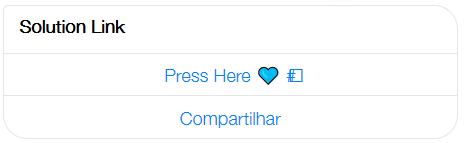
\includegraphics[width=0.7\linewidth]{img/bot1_5.png}
    \caption{Screenshot das opções exibidas pelo MathHook após solucionar um problema matemático.}
    \label{fig:bot1_5}
\end{figure}

A tabela~\ref{tab:bot1} abaixo lista as vantagens e desvantagens que encontrei após um período de conversação com esse chatterbot.
\subsection{ChatterBot MathHook}\label{subsec:bot1}
\input{img/bot1_logo}

Este foi desenvolvido para o aplicativo Messenger do Facebook, assim, pode ser acessado tanto por dispositivos móveis quanto computadores de mesa, desde que tenham o aplicativo instalado. Está atualmente na versão $1.2$ e possui o código aberto, disponível em \url{https://github.com/AhmedMashour/mHookBot}.
Para iniciar uma conversa com ele, basta ir ao seu site \url{http://mathhook.herokuapp.com} ou, encontrá-lo diretamente no aplicativo procurando por ``mathhook''.
Uma pequena demonstração do bot está disponível em vídeo publicado no YouTube no dia 31 de maio de 2017: \url{https://www.youtube.com/watch?v=4f_cMU70TmM}
Esse bot tem como objetivo tanto solucionar problemas matemáticos (soluções bem detalhadas) quanto entregar ao usuário informações que o ajudarão a aprender sobre algo do universo da matemática, oferecendo links de vídeo-aulas e o apoio da comunidade que o compõem.
A linguagem de programação utilizada foi o JavaScript e a língua que o sistema compreende e responde é o Inglês.

A interação com esse chatterbot é unidirecional e se inicia com qualquer mensagem do usuário enviando para ele.
O mesmo responde com mensagens de apresentação (vide a figura~\ref{fig:bot1_1}) e espera que o usuário escolha o que deseja que o bot lhe introduza, que pode ser: soluções, cursos ou acessar a comunidade.
\input{img/bot1_1}

Para prosseguir, escolhi o ramo ``Math Solutions'' a fim de encontrar soluções para alguns problemas matemáticos.
Para tal, bastou selecionar a opção ``Maths Sections''. Como resposta, o bot aguarda novamente uma escolha do usuário. Agora o aspecto é o ramo da aritmética.
\input{img/bot1_2}
O sistema suporta: pré-álgebra, álgebra, matrizes e vetores, funções e gráficos, trigonometria, pré-cálculo, cálculo e estatística (figura~\ref{fig:bot1_2}). 

Ao selecionar ``Equations'' (da categoria ``Pre Calculus''), o bot espera que o usuário faça outra escolha. Agora é sobre o método de equações que ele deseja calcular, podendo escolher entre 8 métodos, tais como: linear, quadrática, logarítmica, etc (figura~\ref{fig:bot1_3}).
\input{img/bot1_3}

Vale ressaltar que durante a conversa, ao digitar uma mensagem que o bot não entende ou enviar uma mensagem quando o bot está esperando a escolha através de um clique em uma das opções, o mesmo responde com a seguinte mensagem interativa (pode ser vista na fig.~\ref{fig:bot1_4}):
\begin{description}
% \item \eu{Foo}
    \item \chatbot{I don't understand what you want try in another form :( Speciy What you meant}
    \item \chatbot{Speciy What you meant}
\end{description}

\input{img/bot1_4}

Continuando a conversação, escolhi o método (equação) Linear, assim, o bot responde (sobrescrevendo a mensagem de escolha dos métodos) com a mensagem abaixo e as opções ``Examples/Exercises'' e ``Detach'' (para interromper):
\begin{description}
    \item \chatbot{Now you're Linked to linear equation calculator. type your problem whenever you want to get examples press the button. Or type examples or detach whenever you want.}
\end{description}
Assim, espera que o usuário envie uma equação linear para ele resolver. Porém, ao escolher se desconectar, o bot continua solucionando os problemas. Além disso, ele também resolve qualquer problema, não estando diretamente relacionado ao método escolhido previamente.

Como meu objetivo é verificar (e validar) a solução encontrada para algum problema, a conversa se seguiu da seguinte forma:
\input{conversas/bot1}
E uma imagem (em baixa qualidade) da solução \emph{correta} etapa-por-etapa da expressão, além das opções ``Press Here'' para verificar melhor a solução e o botão ``Compartilhar'' (fig.~\ref{fig:bot1_5}).
\input{img/bot1_5}

A tabela~\ref{tab:bot1} abaixo lista as vantagens e desvantagens que encontrei após um período de conversação com esse chatterbot.
\input{tables/bot1}

Segue uma lista de melhorias e correções que eu sugiro ao sistema:
\begin{itemize}[noitemsep]
    \item Adicionar uma mensagem de ajuda padrão (e.g., ``help'')
    \item Reduzir o fluxo para os principais objetivos
    \item Permitir que o usuário digite uma das opções e envie como mensagem
    \item Corrigir identificação de expressões em textos (prever erros do usuário)
    \item Detalhar opções que o usuário possui
\end{itemize}

Segue uma lista de melhorias e correções que eu sugiro ao sistema:
\begin{itemize}[noitemsep]
    \item Adicionar uma mensagem de ajuda padrão (e.g., ``help'')
    \item Reduzir o fluxo para os principais objetivos
    \item Permitir que o usuário digite uma das opções e envie como mensagem
    \item Corrigir identificação de expressões em textos (prever erros do usuário)
    \item Detalhar opções que o usuário possui
\end{itemize}

Segue uma lista de melhorias e correções que eu sugiro ao sistema:
\begin{itemize}[noitemsep]
    \item Adicionar uma mensagem de ajuda padrão (e.g., ``help'')
    \item Reduzir o fluxo para os principais objetivos
    \item Permitir que o usuário digite uma das opções e envie como mensagem
    \item Corrigir identificação de expressões em textos (prever erros do usuário)
    \item Detalhar opções que o usuário possui
\end{itemize}
E uma imagem (em baixa qualidade) da solução \emph{correta} etapa-por-etapa da expressão, além das opções ``Press Here'' para verificar melhor a solução e o botão ``Compartilhar'' (fig.~\ref{fig:bot1_5}).
\begin{figure}[h!tbp]
    \centering
    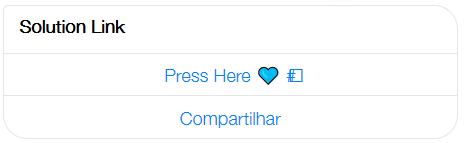
\includegraphics[width=0.7\linewidth]{img/bot1_5.png}
    \caption{Screenshot das opções exibidas pelo MathHook após solucionar um problema matemático.}
    \label{fig:bot1_5}
\end{figure}

A tabela~\ref{tab:bot1} abaixo lista as vantagens e desvantagens que encontrei após um período de conversação com esse chatterbot.
\subsection{ChatterBot MathHook}\label{subsec:bot1}
\begin{figure}[h!tbp]
    \centering
    
\includegraphics[width=0.4\linewidth]{img/bot1_logo.png}
    \caption{Avatar do perfil do MathHook bot.}
    \label{fig:bot1_logo}
\end{figure}

Este foi desenvolvido para o aplicativo Messenger do Facebook, assim, pode ser acessado tanto por dispositivos móveis quanto computadores de mesa, desde que tenham o aplicativo instalado. Está atualmente na versão $1.2$ e possui o código aberto, disponível em \url{https://github.com/AhmedMashour/mHookBot}.
Para iniciar uma conversa com ele, basta ir ao seu site \url{http://mathhook.herokuapp.com} ou, encontrá-lo diretamente no aplicativo procurando por ``mathhook''.
Uma pequena demonstração do bot está disponível em vídeo publicado no YouTube no dia 31 de maio de 2017: \url{https://www.youtube.com/watch?v=4f_cMU70TmM}
Esse bot tem como objetivo tanto solucionar problemas matemáticos (soluções bem detalhadas) quanto entregar ao usuário informações que o ajudarão a aprender sobre algo do universo da matemática, oferecendo links de vídeo-aulas e o apoio da comunidade que o compõem.
A linguagem de programação utilizada foi o JavaScript e a língua que o sistema compreende e responde é o Inglês.

A interação com esse chatterbot é unidirecional e se inicia com qualquer mensagem do usuário enviando para ele.
O mesmo responde com mensagens de apresentação (vide a figura~\ref{fig:bot1_1}) e espera que o usuário escolha o que deseja que o bot lhe introduza, que pode ser: soluções, cursos ou acessar a comunidade.
\begin{figure}[h!tbp]
    \centering
    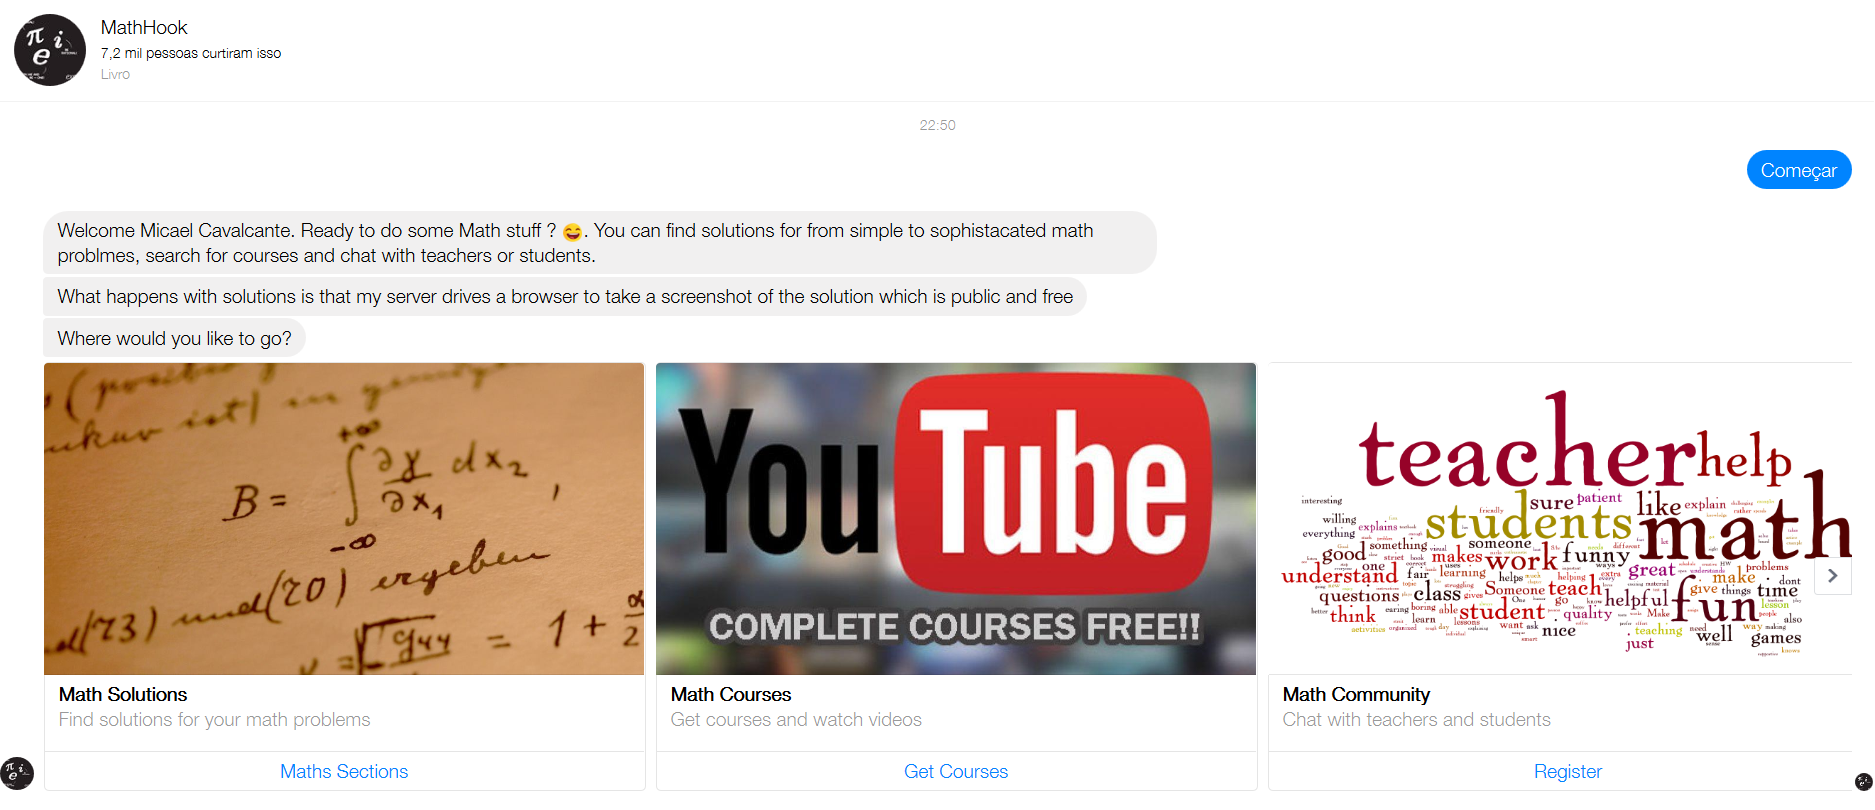
\includegraphics[width=1\linewidth]{img/bot1_1.png}
    \caption{Screenshot do primeiro contato com o MathHook bot.}
    \label{fig:bot1_1}
\end{figure}

Para prosseguir, escolhi o ramo ``Math Solutions'' a fim de encontrar soluções para alguns problemas matemáticos.
Para tal, bastou selecionar a opção ``Maths Sections''. Como resposta, o bot aguarda novamente uma escolha do usuário. Agora o aspecto é o ramo da aritmética.
\begin{figure}[h!tbp]
    \centering
    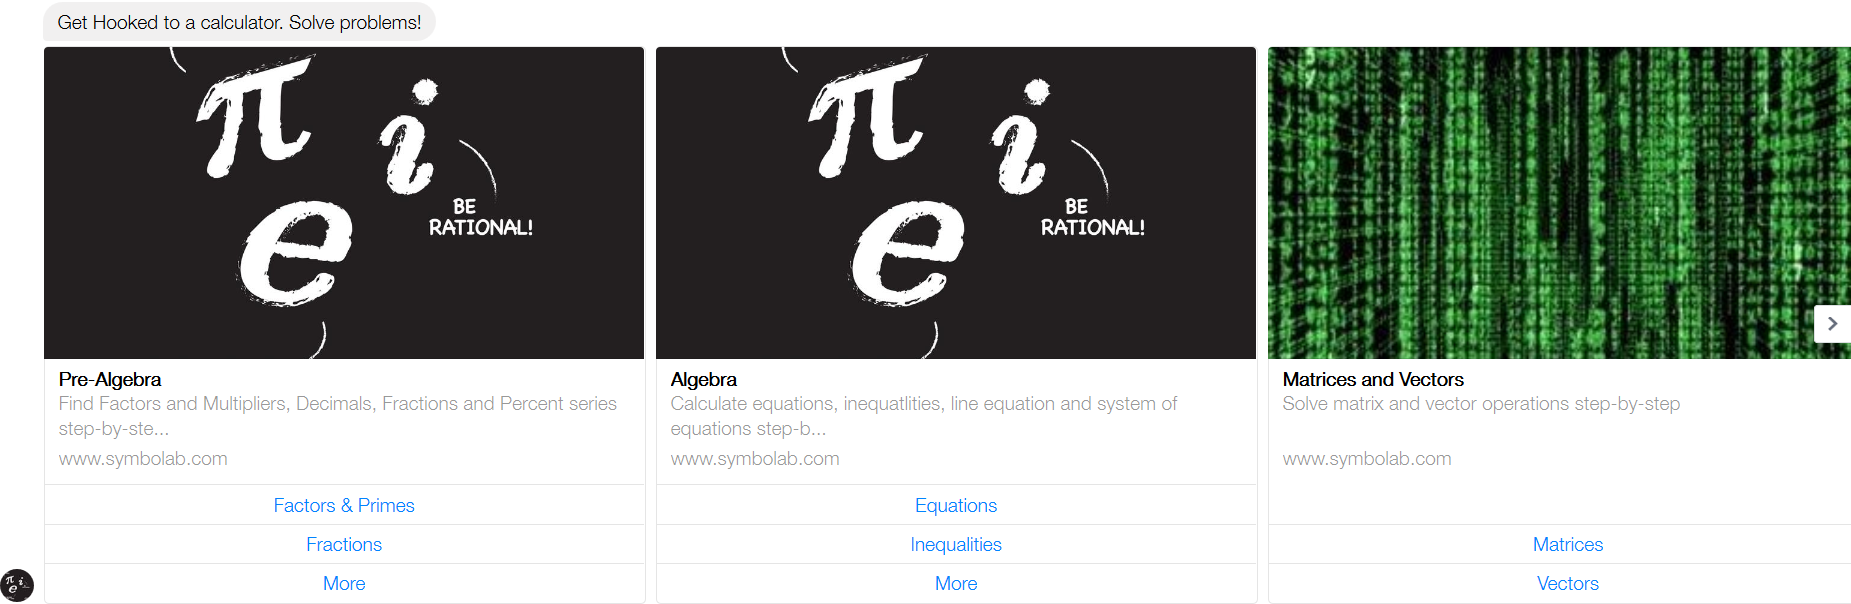
\includegraphics[width=0.65\linewidth]{img/bot1_2.png}
    \caption{Screenshot da resposta do MathHook ao escolher ``Maths Sections''.}
    \label{fig:bot1_2}
\end{figure}
O sistema suporta: pré-álgebra, álgebra, matrizes e vetores, funções e gráficos, trigonometria, pré-cálculo, cálculo e estatística (figura~\ref{fig:bot1_2}). 

Ao selecionar ``Equations'' (da categoria ``Pre Calculus''), o bot espera que o usuário faça outra escolha. Agora é sobre o método de equações que ele deseja calcular, podendo escolher entre 8 métodos, tais como: linear, quadrática, logarítmica, etc (figura~\ref{fig:bot1_3}).
\begin{figure}[h!tbp]
    \centering
    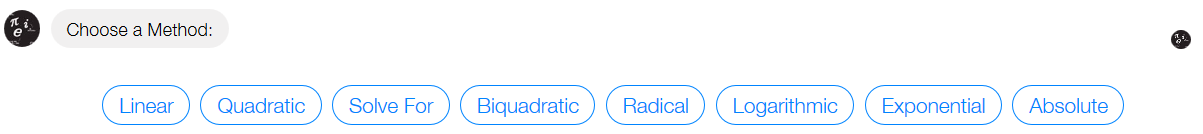
\includegraphics[width=1\linewidth]{img/bot1_3.png}
    \caption{Screenshot da resposta do MathHook ao escolher ``Equations''.}
    \label{fig:bot1_3}
\end{figure}

Vale ressaltar que durante a conversa, ao digitar uma mensagem que o bot não entende ou enviar uma mensagem quando o bot está esperando a escolha através de um clique em uma das opções, o mesmo responde com a seguinte mensagem interativa (pode ser vista na fig.~\ref{fig:bot1_4}):
\begin{description}
% \item \eu{Foo}
    \item \chatbot{I don't understand what you want try in another form :( Speciy What you meant}
    \item \chatbot{Speciy What you meant}
\end{description}

\begin{figure}[h!tbp]
    \centering
    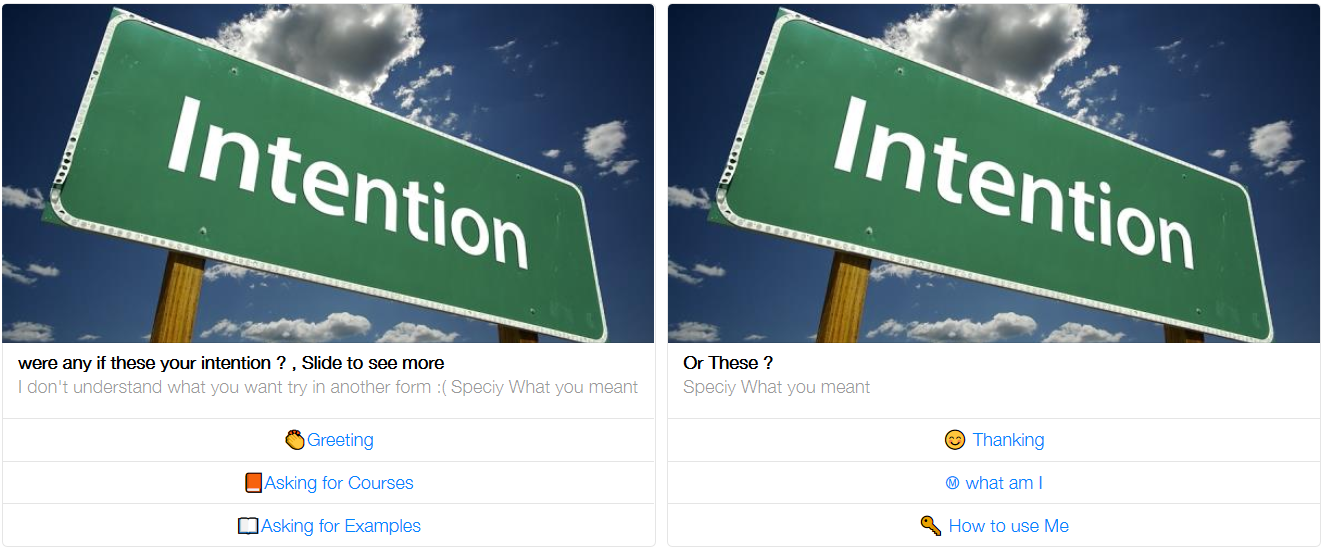
\includegraphics[width=1.1\linewidth]{img/bot1_4.png}
    \caption{Screenshot da resposta do MathHook para mensagens que ele não entende.}
    \label{fig:bot1_4}
\end{figure}

Continuando a conversação, escolhi o método (equação) Linear, assim, o bot responde (sobrescrevendo a mensagem de escolha dos métodos) com a mensagem abaixo e as opções ``Examples/Exercises'' e ``Detach'' (para interromper):
\begin{description}
    \item \chatbot{Now you're Linked to linear equation calculator. type your problem whenever you want to get examples press the button. Or type examples or detach whenever you want.}
\end{description}
Assim, espera que o usuário envie uma equação linear para ele resolver. Porém, ao escolher se desconectar, o bot continua solucionando os problemas. Além disso, ele também resolve qualquer problema, não estando diretamente relacionado ao método escolhido previamente.

Como meu objetivo é verificar (e validar) a solução encontrada para algum problema, a conversa se seguiu da seguinte forma:
\subsection{ChatterBot MathHook}\label{subsec:bot1}
\begin{figure}[h!tbp]
    \centering
    
\includegraphics[width=0.4\linewidth]{img/bot1_logo.png}
    \caption{Avatar do perfil do MathHook bot.}
    \label{fig:bot1_logo}
\end{figure}

Este foi desenvolvido para o aplicativo Messenger do Facebook, assim, pode ser acessado tanto por dispositivos móveis quanto computadores de mesa, desde que tenham o aplicativo instalado. Está atualmente na versão $1.2$ e possui o código aberto, disponível em \url{https://github.com/AhmedMashour/mHookBot}.
Para iniciar uma conversa com ele, basta ir ao seu site \url{http://mathhook.herokuapp.com} ou, encontrá-lo diretamente no aplicativo procurando por ``mathhook''.
Uma pequena demonstração do bot está disponível em vídeo publicado no YouTube no dia 31 de maio de 2017: \url{https://www.youtube.com/watch?v=4f_cMU70TmM}
Esse bot tem como objetivo tanto solucionar problemas matemáticos (soluções bem detalhadas) quanto entregar ao usuário informações que o ajudarão a aprender sobre algo do universo da matemática, oferecendo links de vídeo-aulas e o apoio da comunidade que o compõem.
A linguagem de programação utilizada foi o JavaScript e a língua que o sistema compreende e responde é o Inglês.

A interação com esse chatterbot é unidirecional e se inicia com qualquer mensagem do usuário enviando para ele.
O mesmo responde com mensagens de apresentação (vide a figura~\ref{fig:bot1_1}) e espera que o usuário escolha o que deseja que o bot lhe introduza, que pode ser: soluções, cursos ou acessar a comunidade.
\begin{figure}[h!tbp]
    \centering
    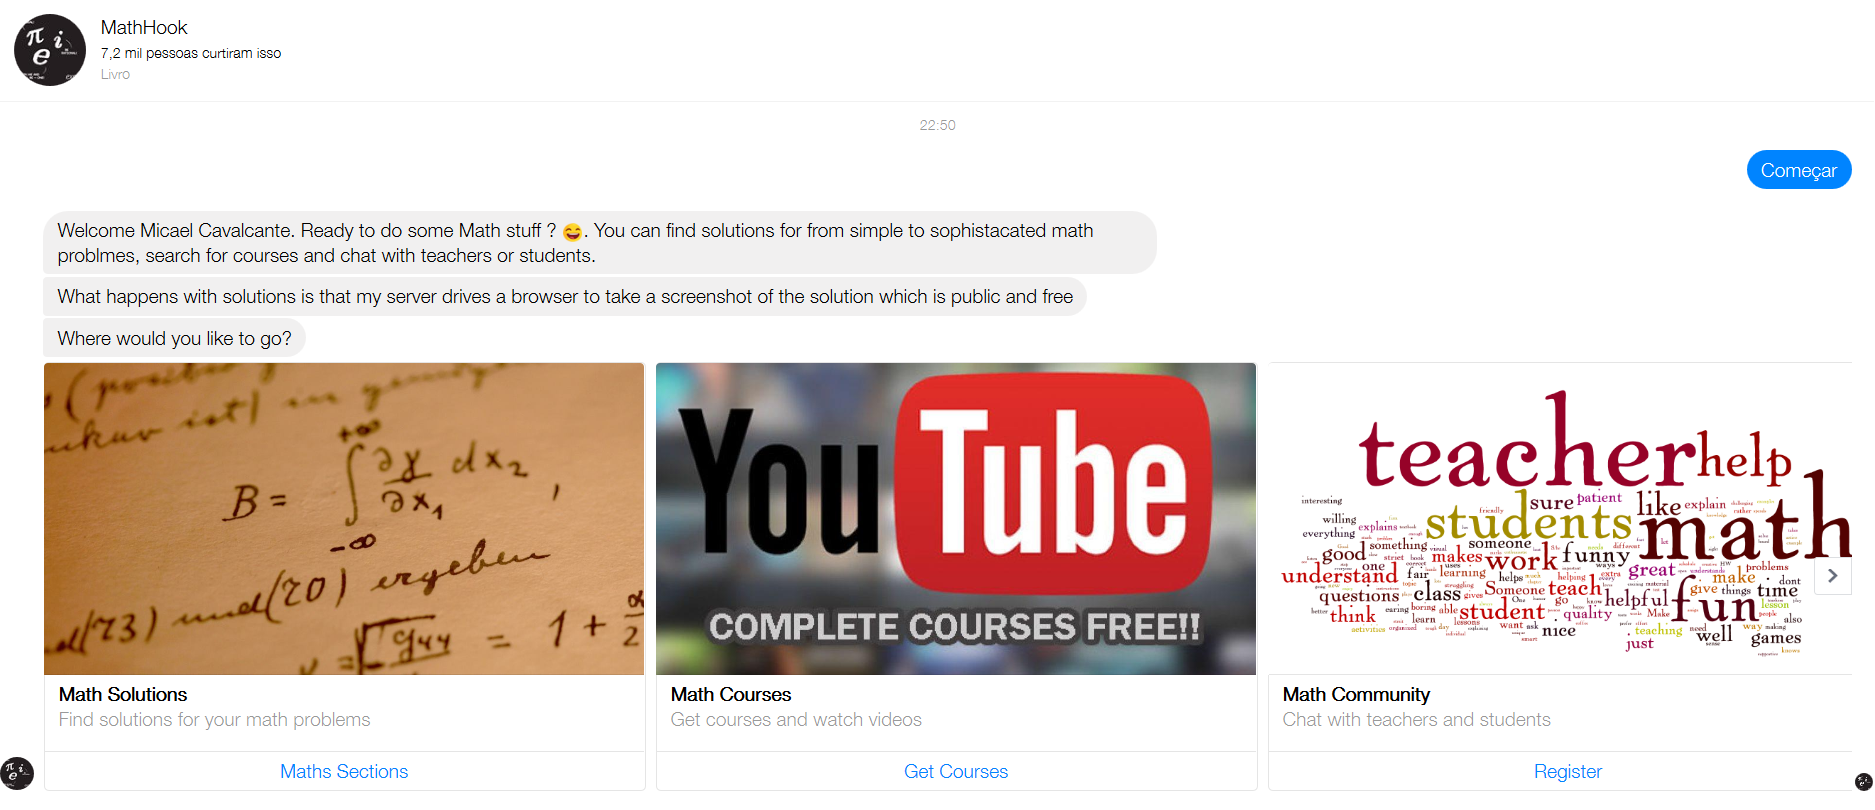
\includegraphics[width=1\linewidth]{img/bot1_1.png}
    \caption{Screenshot do primeiro contato com o MathHook bot.}
    \label{fig:bot1_1}
\end{figure}

Para prosseguir, escolhi o ramo ``Math Solutions'' a fim de encontrar soluções para alguns problemas matemáticos.
Para tal, bastou selecionar a opção ``Maths Sections''. Como resposta, o bot aguarda novamente uma escolha do usuário. Agora o aspecto é o ramo da aritmética.
\begin{figure}[h!tbp]
    \centering
    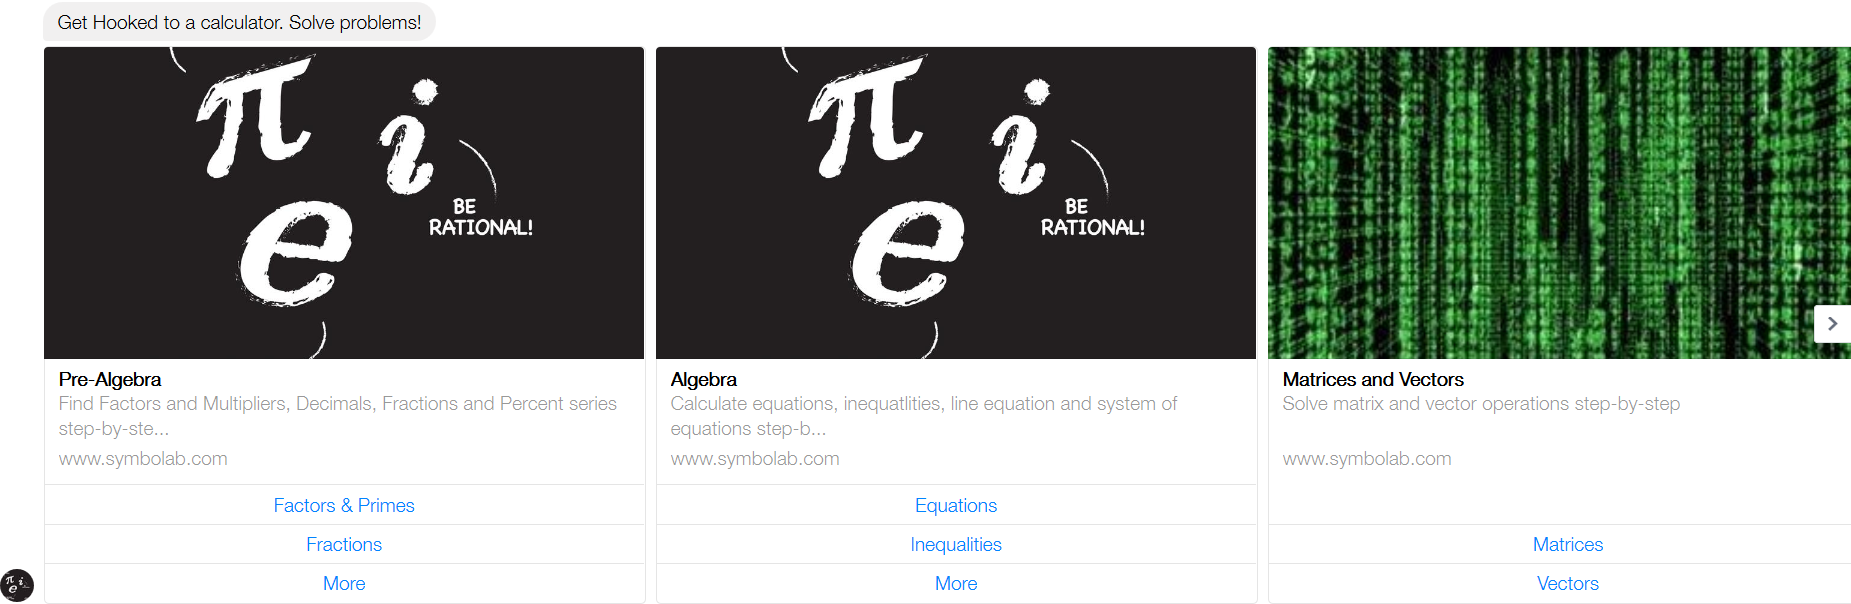
\includegraphics[width=0.65\linewidth]{img/bot1_2.png}
    \caption{Screenshot da resposta do MathHook ao escolher ``Maths Sections''.}
    \label{fig:bot1_2}
\end{figure}
O sistema suporta: pré-álgebra, álgebra, matrizes e vetores, funções e gráficos, trigonometria, pré-cálculo, cálculo e estatística (figura~\ref{fig:bot1_2}). 

Ao selecionar ``Equations'' (da categoria ``Pre Calculus''), o bot espera que o usuário faça outra escolha. Agora é sobre o método de equações que ele deseja calcular, podendo escolher entre 8 métodos, tais como: linear, quadrática, logarítmica, etc (figura~\ref{fig:bot1_3}).
\begin{figure}[h!tbp]
    \centering
    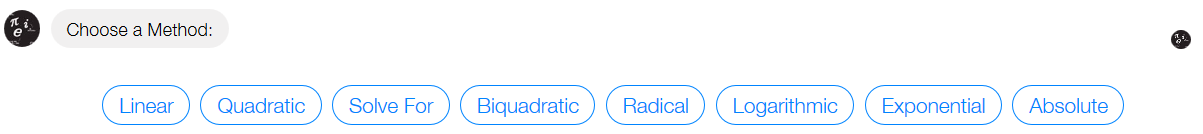
\includegraphics[width=1\linewidth]{img/bot1_3.png}
    \caption{Screenshot da resposta do MathHook ao escolher ``Equations''.}
    \label{fig:bot1_3}
\end{figure}

Vale ressaltar que durante a conversa, ao digitar uma mensagem que o bot não entende ou enviar uma mensagem quando o bot está esperando a escolha através de um clique em uma das opções, o mesmo responde com a seguinte mensagem interativa (pode ser vista na fig.~\ref{fig:bot1_4}):
\begin{description}
% \item \eu{Foo}
    \item \chatbot{I don't understand what you want try in another form :( Speciy What you meant}
    \item \chatbot{Speciy What you meant}
\end{description}

\begin{figure}[h!tbp]
    \centering
    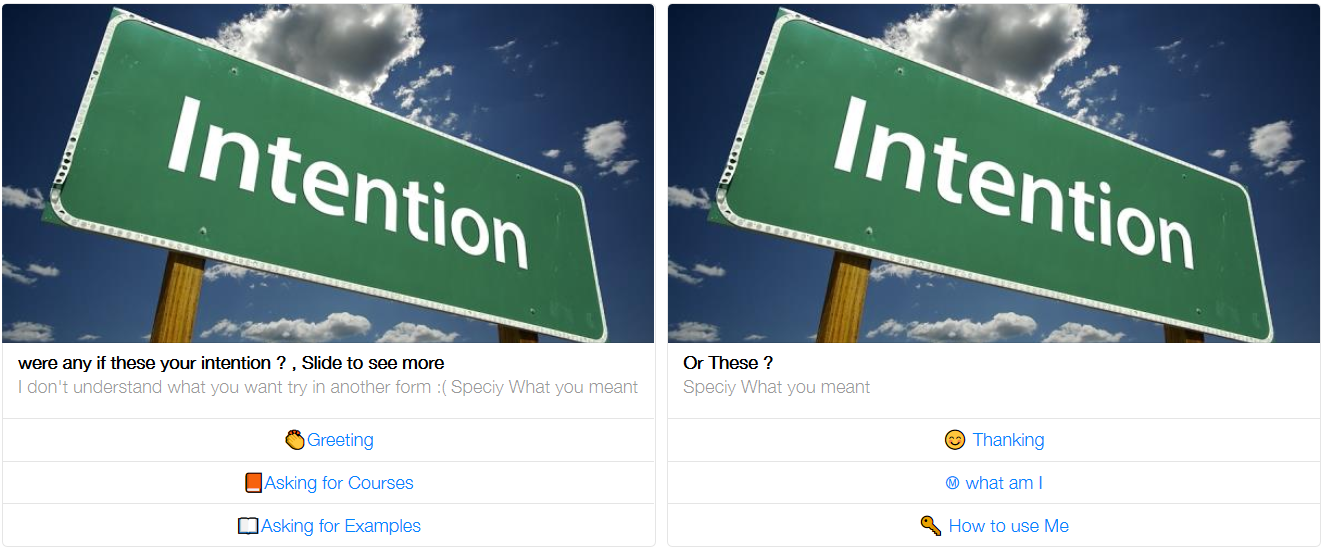
\includegraphics[width=1.1\linewidth]{img/bot1_4.png}
    \caption{Screenshot da resposta do MathHook para mensagens que ele não entende.}
    \label{fig:bot1_4}
\end{figure}

Continuando a conversação, escolhi o método (equação) Linear, assim, o bot responde (sobrescrevendo a mensagem de escolha dos métodos) com a mensagem abaixo e as opções ``Examples/Exercises'' e ``Detach'' (para interromper):
\begin{description}
    \item \chatbot{Now you're Linked to linear equation calculator. type your problem whenever you want to get examples press the button. Or type examples or detach whenever you want.}
\end{description}
Assim, espera que o usuário envie uma equação linear para ele resolver. Porém, ao escolher se desconectar, o bot continua solucionando os problemas. Além disso, ele também resolve qualquer problema, não estando diretamente relacionado ao método escolhido previamente.

Como meu objetivo é verificar (e validar) a solução encontrada para algum problema, a conversa se seguiu da seguinte forma:
\subsection{ChatterBot MathHook}\label{subsec:bot1}
\input{img/bot1_logo}

Este foi desenvolvido para o aplicativo Messenger do Facebook, assim, pode ser acessado tanto por dispositivos móveis quanto computadores de mesa, desde que tenham o aplicativo instalado. Está atualmente na versão $1.2$ e possui o código aberto, disponível em \url{https://github.com/AhmedMashour/mHookBot}.
Para iniciar uma conversa com ele, basta ir ao seu site \url{http://mathhook.herokuapp.com} ou, encontrá-lo diretamente no aplicativo procurando por ``mathhook''.
Uma pequena demonstração do bot está disponível em vídeo publicado no YouTube no dia 31 de maio de 2017: \url{https://www.youtube.com/watch?v=4f_cMU70TmM}
Esse bot tem como objetivo tanto solucionar problemas matemáticos (soluções bem detalhadas) quanto entregar ao usuário informações que o ajudarão a aprender sobre algo do universo da matemática, oferecendo links de vídeo-aulas e o apoio da comunidade que o compõem.
A linguagem de programação utilizada foi o JavaScript e a língua que o sistema compreende e responde é o Inglês.

A interação com esse chatterbot é unidirecional e se inicia com qualquer mensagem do usuário enviando para ele.
O mesmo responde com mensagens de apresentação (vide a figura~\ref{fig:bot1_1}) e espera que o usuário escolha o que deseja que o bot lhe introduza, que pode ser: soluções, cursos ou acessar a comunidade.
\input{img/bot1_1}

Para prosseguir, escolhi o ramo ``Math Solutions'' a fim de encontrar soluções para alguns problemas matemáticos.
Para tal, bastou selecionar a opção ``Maths Sections''. Como resposta, o bot aguarda novamente uma escolha do usuário. Agora o aspecto é o ramo da aritmética.
\input{img/bot1_2}
O sistema suporta: pré-álgebra, álgebra, matrizes e vetores, funções e gráficos, trigonometria, pré-cálculo, cálculo e estatística (figura~\ref{fig:bot1_2}). 

Ao selecionar ``Equations'' (da categoria ``Pre Calculus''), o bot espera que o usuário faça outra escolha. Agora é sobre o método de equações que ele deseja calcular, podendo escolher entre 8 métodos, tais como: linear, quadrática, logarítmica, etc (figura~\ref{fig:bot1_3}).
\input{img/bot1_3}

Vale ressaltar que durante a conversa, ao digitar uma mensagem que o bot não entende ou enviar uma mensagem quando o bot está esperando a escolha através de um clique em uma das opções, o mesmo responde com a seguinte mensagem interativa (pode ser vista na fig.~\ref{fig:bot1_4}):
\begin{description}
% \item \eu{Foo}
    \item \chatbot{I don't understand what you want try in another form :( Speciy What you meant}
    \item \chatbot{Speciy What you meant}
\end{description}

\input{img/bot1_4}

Continuando a conversação, escolhi o método (equação) Linear, assim, o bot responde (sobrescrevendo a mensagem de escolha dos métodos) com a mensagem abaixo e as opções ``Examples/Exercises'' e ``Detach'' (para interromper):
\begin{description}
    \item \chatbot{Now you're Linked to linear equation calculator. type your problem whenever you want to get examples press the button. Or type examples or detach whenever you want.}
\end{description}
Assim, espera que o usuário envie uma equação linear para ele resolver. Porém, ao escolher se desconectar, o bot continua solucionando os problemas. Além disso, ele também resolve qualquer problema, não estando diretamente relacionado ao método escolhido previamente.

Como meu objetivo é verificar (e validar) a solução encontrada para algum problema, a conversa se seguiu da seguinte forma:
\input{conversas/bot1}
E uma imagem (em baixa qualidade) da solução \emph{correta} etapa-por-etapa da expressão, além das opções ``Press Here'' para verificar melhor a solução e o botão ``Compartilhar'' (fig.~\ref{fig:bot1_5}).
\input{img/bot1_5}

A tabela~\ref{tab:bot1} abaixo lista as vantagens e desvantagens que encontrei após um período de conversação com esse chatterbot.
\input{tables/bot1}

Segue uma lista de melhorias e correções que eu sugiro ao sistema:
\begin{itemize}[noitemsep]
    \item Adicionar uma mensagem de ajuda padrão (e.g., ``help'')
    \item Reduzir o fluxo para os principais objetivos
    \item Permitir que o usuário digite uma das opções e envie como mensagem
    \item Corrigir identificação de expressões em textos (prever erros do usuário)
    \item Detalhar opções que o usuário possui
\end{itemize}
E uma imagem (em baixa qualidade) da solução \emph{correta} etapa-por-etapa da expressão, além das opções ``Press Here'' para verificar melhor a solução e o botão ``Compartilhar'' (fig.~\ref{fig:bot1_5}).
\begin{figure}[h!tbp]
    \centering
    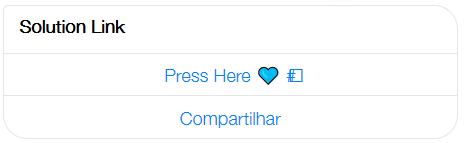
\includegraphics[width=0.7\linewidth]{img/bot1_5.png}
    \caption{Screenshot das opções exibidas pelo MathHook após solucionar um problema matemático.}
    \label{fig:bot1_5}
\end{figure}

A tabela~\ref{tab:bot1} abaixo lista as vantagens e desvantagens que encontrei após um período de conversação com esse chatterbot.
\subsection{ChatterBot MathHook}\label{subsec:bot1}
\input{img/bot1_logo}

Este foi desenvolvido para o aplicativo Messenger do Facebook, assim, pode ser acessado tanto por dispositivos móveis quanto computadores de mesa, desde que tenham o aplicativo instalado. Está atualmente na versão $1.2$ e possui o código aberto, disponível em \url{https://github.com/AhmedMashour/mHookBot}.
Para iniciar uma conversa com ele, basta ir ao seu site \url{http://mathhook.herokuapp.com} ou, encontrá-lo diretamente no aplicativo procurando por ``mathhook''.
Uma pequena demonstração do bot está disponível em vídeo publicado no YouTube no dia 31 de maio de 2017: \url{https://www.youtube.com/watch?v=4f_cMU70TmM}
Esse bot tem como objetivo tanto solucionar problemas matemáticos (soluções bem detalhadas) quanto entregar ao usuário informações que o ajudarão a aprender sobre algo do universo da matemática, oferecendo links de vídeo-aulas e o apoio da comunidade que o compõem.
A linguagem de programação utilizada foi o JavaScript e a língua que o sistema compreende e responde é o Inglês.

A interação com esse chatterbot é unidirecional e se inicia com qualquer mensagem do usuário enviando para ele.
O mesmo responde com mensagens de apresentação (vide a figura~\ref{fig:bot1_1}) e espera que o usuário escolha o que deseja que o bot lhe introduza, que pode ser: soluções, cursos ou acessar a comunidade.
\input{img/bot1_1}

Para prosseguir, escolhi o ramo ``Math Solutions'' a fim de encontrar soluções para alguns problemas matemáticos.
Para tal, bastou selecionar a opção ``Maths Sections''. Como resposta, o bot aguarda novamente uma escolha do usuário. Agora o aspecto é o ramo da aritmética.
\input{img/bot1_2}
O sistema suporta: pré-álgebra, álgebra, matrizes e vetores, funções e gráficos, trigonometria, pré-cálculo, cálculo e estatística (figura~\ref{fig:bot1_2}). 

Ao selecionar ``Equations'' (da categoria ``Pre Calculus''), o bot espera que o usuário faça outra escolha. Agora é sobre o método de equações que ele deseja calcular, podendo escolher entre 8 métodos, tais como: linear, quadrática, logarítmica, etc (figura~\ref{fig:bot1_3}).
\input{img/bot1_3}

Vale ressaltar que durante a conversa, ao digitar uma mensagem que o bot não entende ou enviar uma mensagem quando o bot está esperando a escolha através de um clique em uma das opções, o mesmo responde com a seguinte mensagem interativa (pode ser vista na fig.~\ref{fig:bot1_4}):
\begin{description}
% \item \eu{Foo}
    \item \chatbot{I don't understand what you want try in another form :( Speciy What you meant}
    \item \chatbot{Speciy What you meant}
\end{description}

\input{img/bot1_4}

Continuando a conversação, escolhi o método (equação) Linear, assim, o bot responde (sobrescrevendo a mensagem de escolha dos métodos) com a mensagem abaixo e as opções ``Examples/Exercises'' e ``Detach'' (para interromper):
\begin{description}
    \item \chatbot{Now you're Linked to linear equation calculator. type your problem whenever you want to get examples press the button. Or type examples or detach whenever you want.}
\end{description}
Assim, espera que o usuário envie uma equação linear para ele resolver. Porém, ao escolher se desconectar, o bot continua solucionando os problemas. Além disso, ele também resolve qualquer problema, não estando diretamente relacionado ao método escolhido previamente.

Como meu objetivo é verificar (e validar) a solução encontrada para algum problema, a conversa se seguiu da seguinte forma:
\input{conversas/bot1}
E uma imagem (em baixa qualidade) da solução \emph{correta} etapa-por-etapa da expressão, além das opções ``Press Here'' para verificar melhor a solução e o botão ``Compartilhar'' (fig.~\ref{fig:bot1_5}).
\input{img/bot1_5}

A tabela~\ref{tab:bot1} abaixo lista as vantagens e desvantagens que encontrei após um período de conversação com esse chatterbot.
\input{tables/bot1}

Segue uma lista de melhorias e correções que eu sugiro ao sistema:
\begin{itemize}[noitemsep]
    \item Adicionar uma mensagem de ajuda padrão (e.g., ``help'')
    \item Reduzir o fluxo para os principais objetivos
    \item Permitir que o usuário digite uma das opções e envie como mensagem
    \item Corrigir identificação de expressões em textos (prever erros do usuário)
    \item Detalhar opções que o usuário possui
\end{itemize}

Segue uma lista de melhorias e correções que eu sugiro ao sistema:
\begin{itemize}[noitemsep]
    \item Adicionar uma mensagem de ajuda padrão (e.g., ``help'')
    \item Reduzir o fluxo para os principais objetivos
    \item Permitir que o usuário digite uma das opções e envie como mensagem
    \item Corrigir identificação de expressões em textos (prever erros do usuário)
    \item Detalhar opções que o usuário possui
\end{itemize}
E uma imagem (em baixa qualidade) da solução \emph{correta} etapa-por-etapa da expressão, além das opções ``Press Here'' para verificar melhor a solução e o botão ``Compartilhar'' (fig.~\ref{fig:bot1_5}).
\begin{figure}[h!tbp]
    \centering
    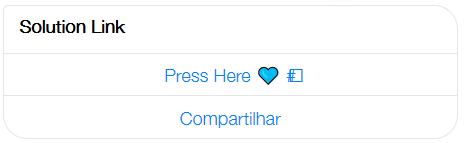
\includegraphics[width=0.7\linewidth]{img/bot1_5.png}
    \caption{Screenshot das opções exibidas pelo MathHook após solucionar um problema matemático.}
    \label{fig:bot1_5}
\end{figure}

A tabela~\ref{tab:bot1} abaixo lista as vantagens e desvantagens que encontrei após um período de conversação com esse chatterbot.
\subsection{ChatterBot MathHook}\label{subsec:bot1}
\begin{figure}[h!tbp]
    \centering
    
\includegraphics[width=0.4\linewidth]{img/bot1_logo.png}
    \caption{Avatar do perfil do MathHook bot.}
    \label{fig:bot1_logo}
\end{figure}

Este foi desenvolvido para o aplicativo Messenger do Facebook, assim, pode ser acessado tanto por dispositivos móveis quanto computadores de mesa, desde que tenham o aplicativo instalado. Está atualmente na versão $1.2$ e possui o código aberto, disponível em \url{https://github.com/AhmedMashour/mHookBot}.
Para iniciar uma conversa com ele, basta ir ao seu site \url{http://mathhook.herokuapp.com} ou, encontrá-lo diretamente no aplicativo procurando por ``mathhook''.
Uma pequena demonstração do bot está disponível em vídeo publicado no YouTube no dia 31 de maio de 2017: \url{https://www.youtube.com/watch?v=4f_cMU70TmM}
Esse bot tem como objetivo tanto solucionar problemas matemáticos (soluções bem detalhadas) quanto entregar ao usuário informações que o ajudarão a aprender sobre algo do universo da matemática, oferecendo links de vídeo-aulas e o apoio da comunidade que o compõem.
A linguagem de programação utilizada foi o JavaScript e a língua que o sistema compreende e responde é o Inglês.

A interação com esse chatterbot é unidirecional e se inicia com qualquer mensagem do usuário enviando para ele.
O mesmo responde com mensagens de apresentação (vide a figura~\ref{fig:bot1_1}) e espera que o usuário escolha o que deseja que o bot lhe introduza, que pode ser: soluções, cursos ou acessar a comunidade.
\begin{figure}[h!tbp]
    \centering
    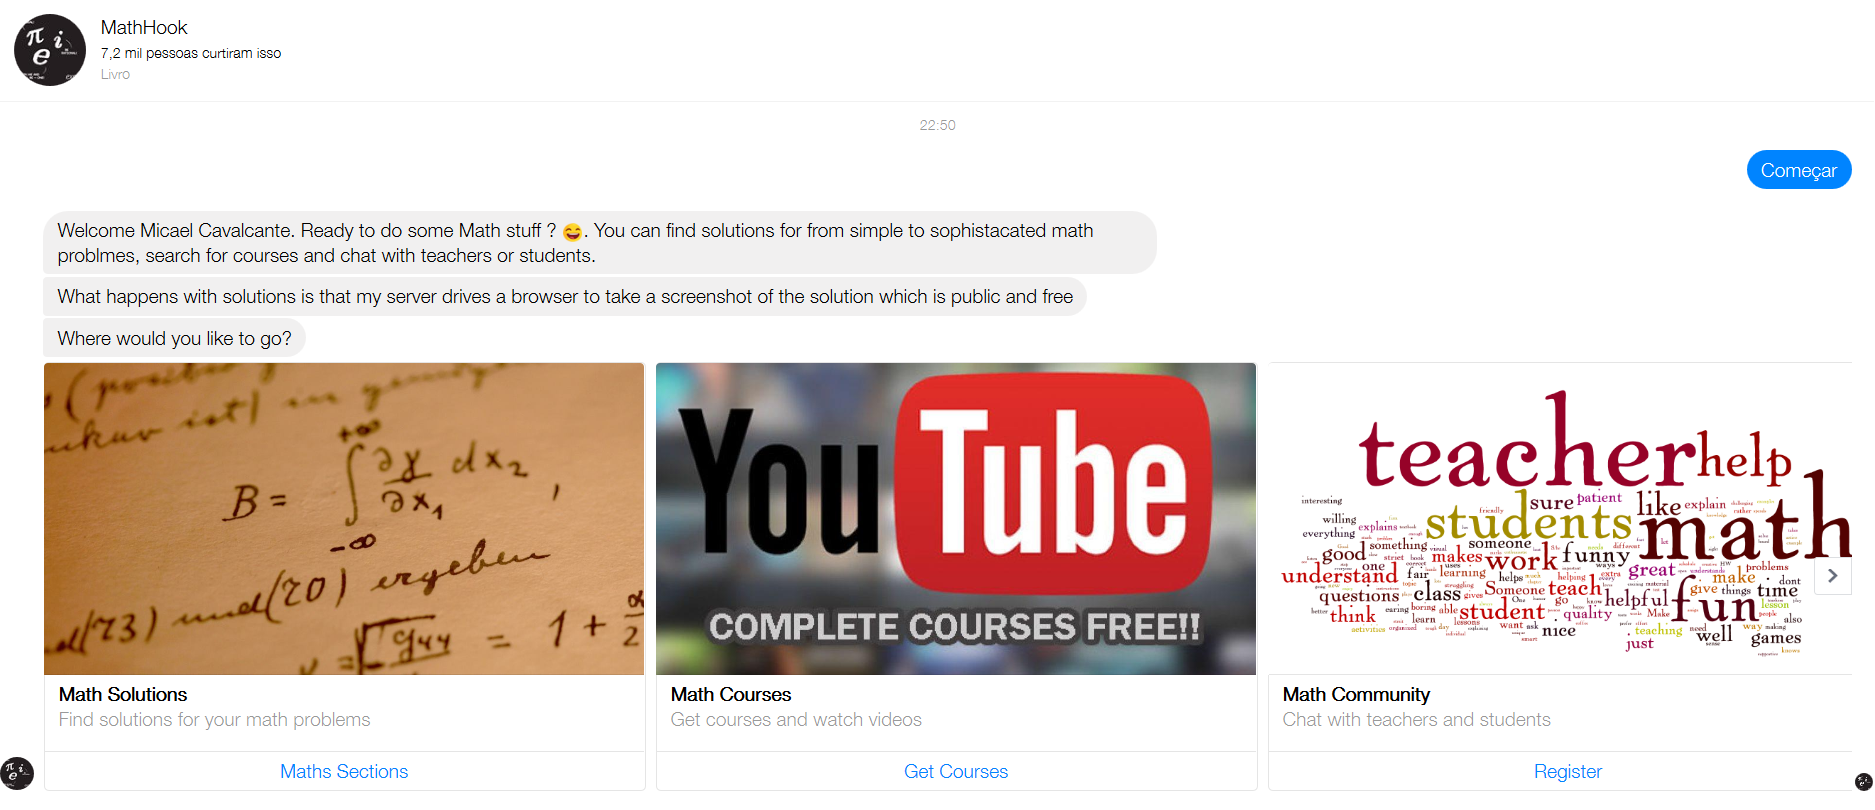
\includegraphics[width=1\linewidth]{img/bot1_1.png}
    \caption{Screenshot do primeiro contato com o MathHook bot.}
    \label{fig:bot1_1}
\end{figure}

Para prosseguir, escolhi o ramo ``Math Solutions'' a fim de encontrar soluções para alguns problemas matemáticos.
Para tal, bastou selecionar a opção ``Maths Sections''. Como resposta, o bot aguarda novamente uma escolha do usuário. Agora o aspecto é o ramo da aritmética.
\begin{figure}[h!tbp]
    \centering
    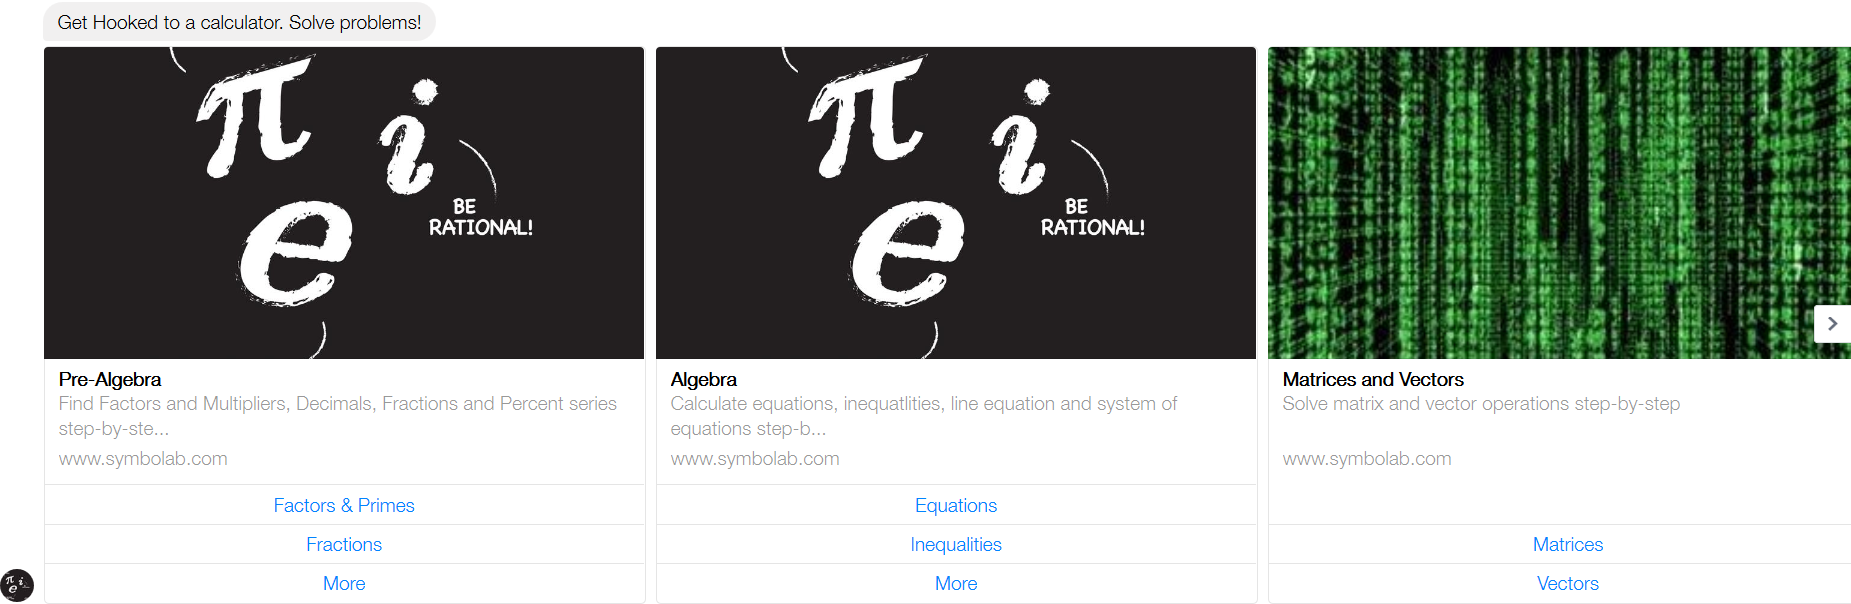
\includegraphics[width=0.65\linewidth]{img/bot1_2.png}
    \caption{Screenshot da resposta do MathHook ao escolher ``Maths Sections''.}
    \label{fig:bot1_2}
\end{figure}
O sistema suporta: pré-álgebra, álgebra, matrizes e vetores, funções e gráficos, trigonometria, pré-cálculo, cálculo e estatística (figura~\ref{fig:bot1_2}). 

Ao selecionar ``Equations'' (da categoria ``Pre Calculus''), o bot espera que o usuário faça outra escolha. Agora é sobre o método de equações que ele deseja calcular, podendo escolher entre 8 métodos, tais como: linear, quadrática, logarítmica, etc (figura~\ref{fig:bot1_3}).
\begin{figure}[h!tbp]
    \centering
    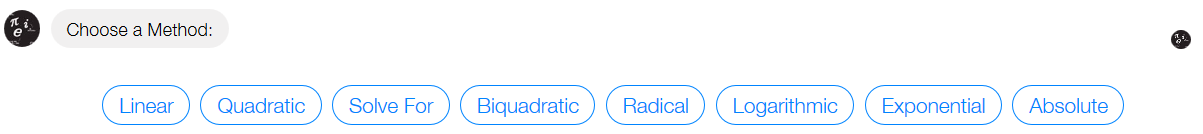
\includegraphics[width=1\linewidth]{img/bot1_3.png}
    \caption{Screenshot da resposta do MathHook ao escolher ``Equations''.}
    \label{fig:bot1_3}
\end{figure}

Vale ressaltar que durante a conversa, ao digitar uma mensagem que o bot não entende ou enviar uma mensagem quando o bot está esperando a escolha através de um clique em uma das opções, o mesmo responde com a seguinte mensagem interativa (pode ser vista na fig.~\ref{fig:bot1_4}):
\begin{description}
% \item \eu{Foo}
    \item \chatbot{I don't understand what you want try in another form :( Speciy What you meant}
    \item \chatbot{Speciy What you meant}
\end{description}

\begin{figure}[h!tbp]
    \centering
    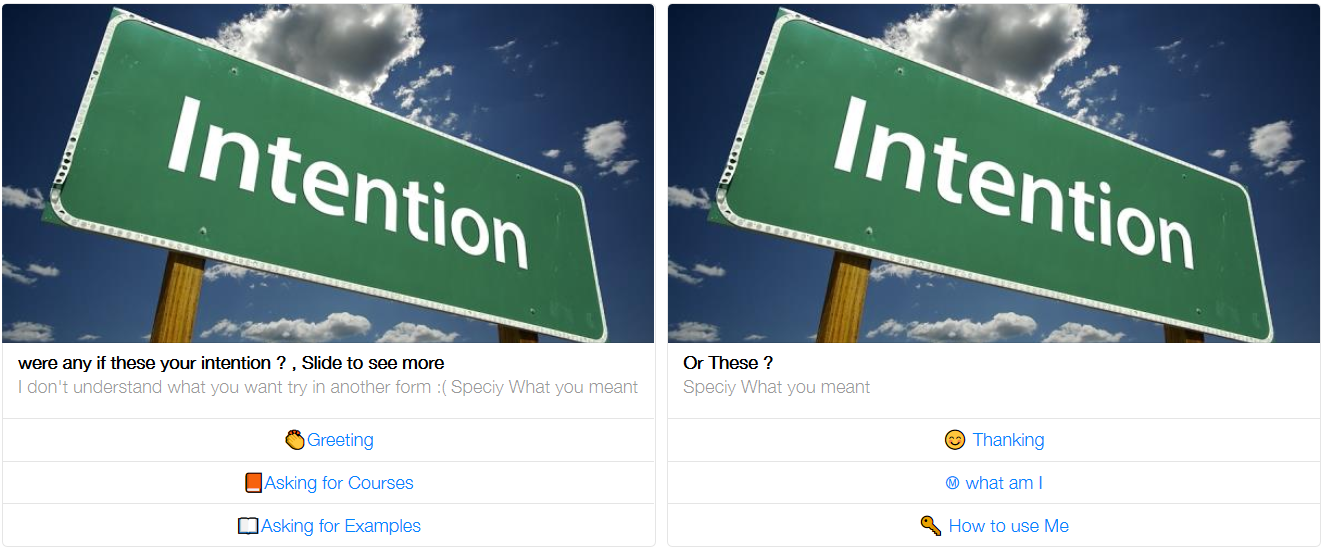
\includegraphics[width=1.1\linewidth]{img/bot1_4.png}
    \caption{Screenshot da resposta do MathHook para mensagens que ele não entende.}
    \label{fig:bot1_4}
\end{figure}

Continuando a conversação, escolhi o método (equação) Linear, assim, o bot responde (sobrescrevendo a mensagem de escolha dos métodos) com a mensagem abaixo e as opções ``Examples/Exercises'' e ``Detach'' (para interromper):
\begin{description}
    \item \chatbot{Now you're Linked to linear equation calculator. type your problem whenever you want to get examples press the button. Or type examples or detach whenever you want.}
\end{description}
Assim, espera que o usuário envie uma equação linear para ele resolver. Porém, ao escolher se desconectar, o bot continua solucionando os problemas. Além disso, ele também resolve qualquer problema, não estando diretamente relacionado ao método escolhido previamente.

Como meu objetivo é verificar (e validar) a solução encontrada para algum problema, a conversa se seguiu da seguinte forma:
\subsection{ChatterBot MathHook}\label{subsec:bot1}
\input{img/bot1_logo}

Este foi desenvolvido para o aplicativo Messenger do Facebook, assim, pode ser acessado tanto por dispositivos móveis quanto computadores de mesa, desde que tenham o aplicativo instalado. Está atualmente na versão $1.2$ e possui o código aberto, disponível em \url{https://github.com/AhmedMashour/mHookBot}.
Para iniciar uma conversa com ele, basta ir ao seu site \url{http://mathhook.herokuapp.com} ou, encontrá-lo diretamente no aplicativo procurando por ``mathhook''.
Uma pequena demonstração do bot está disponível em vídeo publicado no YouTube no dia 31 de maio de 2017: \url{https://www.youtube.com/watch?v=4f_cMU70TmM}
Esse bot tem como objetivo tanto solucionar problemas matemáticos (soluções bem detalhadas) quanto entregar ao usuário informações que o ajudarão a aprender sobre algo do universo da matemática, oferecendo links de vídeo-aulas e o apoio da comunidade que o compõem.
A linguagem de programação utilizada foi o JavaScript e a língua que o sistema compreende e responde é o Inglês.

A interação com esse chatterbot é unidirecional e se inicia com qualquer mensagem do usuário enviando para ele.
O mesmo responde com mensagens de apresentação (vide a figura~\ref{fig:bot1_1}) e espera que o usuário escolha o que deseja que o bot lhe introduza, que pode ser: soluções, cursos ou acessar a comunidade.
\input{img/bot1_1}

Para prosseguir, escolhi o ramo ``Math Solutions'' a fim de encontrar soluções para alguns problemas matemáticos.
Para tal, bastou selecionar a opção ``Maths Sections''. Como resposta, o bot aguarda novamente uma escolha do usuário. Agora o aspecto é o ramo da aritmética.
\input{img/bot1_2}
O sistema suporta: pré-álgebra, álgebra, matrizes e vetores, funções e gráficos, trigonometria, pré-cálculo, cálculo e estatística (figura~\ref{fig:bot1_2}). 

Ao selecionar ``Equations'' (da categoria ``Pre Calculus''), o bot espera que o usuário faça outra escolha. Agora é sobre o método de equações que ele deseja calcular, podendo escolher entre 8 métodos, tais como: linear, quadrática, logarítmica, etc (figura~\ref{fig:bot1_3}).
\input{img/bot1_3}

Vale ressaltar que durante a conversa, ao digitar uma mensagem que o bot não entende ou enviar uma mensagem quando o bot está esperando a escolha através de um clique em uma das opções, o mesmo responde com a seguinte mensagem interativa (pode ser vista na fig.~\ref{fig:bot1_4}):
\begin{description}
% \item \eu{Foo}
    \item \chatbot{I don't understand what you want try in another form :( Speciy What you meant}
    \item \chatbot{Speciy What you meant}
\end{description}

\input{img/bot1_4}

Continuando a conversação, escolhi o método (equação) Linear, assim, o bot responde (sobrescrevendo a mensagem de escolha dos métodos) com a mensagem abaixo e as opções ``Examples/Exercises'' e ``Detach'' (para interromper):
\begin{description}
    \item \chatbot{Now you're Linked to linear equation calculator. type your problem whenever you want to get examples press the button. Or type examples or detach whenever you want.}
\end{description}
Assim, espera que o usuário envie uma equação linear para ele resolver. Porém, ao escolher se desconectar, o bot continua solucionando os problemas. Além disso, ele também resolve qualquer problema, não estando diretamente relacionado ao método escolhido previamente.

Como meu objetivo é verificar (e validar) a solução encontrada para algum problema, a conversa se seguiu da seguinte forma:
\input{conversas/bot1}
E uma imagem (em baixa qualidade) da solução \emph{correta} etapa-por-etapa da expressão, além das opções ``Press Here'' para verificar melhor a solução e o botão ``Compartilhar'' (fig.~\ref{fig:bot1_5}).
\input{img/bot1_5}

A tabela~\ref{tab:bot1} abaixo lista as vantagens e desvantagens que encontrei após um período de conversação com esse chatterbot.
\input{tables/bot1}

Segue uma lista de melhorias e correções que eu sugiro ao sistema:
\begin{itemize}[noitemsep]
    \item Adicionar uma mensagem de ajuda padrão (e.g., ``help'')
    \item Reduzir o fluxo para os principais objetivos
    \item Permitir que o usuário digite uma das opções e envie como mensagem
    \item Corrigir identificação de expressões em textos (prever erros do usuário)
    \item Detalhar opções que o usuário possui
\end{itemize}
E uma imagem (em baixa qualidade) da solução \emph{correta} etapa-por-etapa da expressão, além das opções ``Press Here'' para verificar melhor a solução e o botão ``Compartilhar'' (fig.~\ref{fig:bot1_5}).
\begin{figure}[h!tbp]
    \centering
    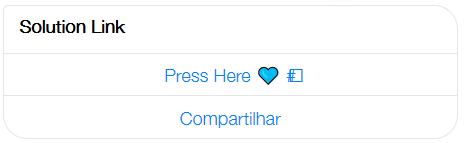
\includegraphics[width=0.7\linewidth]{img/bot1_5.png}
    \caption{Screenshot das opções exibidas pelo MathHook após solucionar um problema matemático.}
    \label{fig:bot1_5}
\end{figure}

A tabela~\ref{tab:bot1} abaixo lista as vantagens e desvantagens que encontrei após um período de conversação com esse chatterbot.
\subsection{ChatterBot MathHook}\label{subsec:bot1}
\input{img/bot1_logo}

Este foi desenvolvido para o aplicativo Messenger do Facebook, assim, pode ser acessado tanto por dispositivos móveis quanto computadores de mesa, desde que tenham o aplicativo instalado. Está atualmente na versão $1.2$ e possui o código aberto, disponível em \url{https://github.com/AhmedMashour/mHookBot}.
Para iniciar uma conversa com ele, basta ir ao seu site \url{http://mathhook.herokuapp.com} ou, encontrá-lo diretamente no aplicativo procurando por ``mathhook''.
Uma pequena demonstração do bot está disponível em vídeo publicado no YouTube no dia 31 de maio de 2017: \url{https://www.youtube.com/watch?v=4f_cMU70TmM}
Esse bot tem como objetivo tanto solucionar problemas matemáticos (soluções bem detalhadas) quanto entregar ao usuário informações que o ajudarão a aprender sobre algo do universo da matemática, oferecendo links de vídeo-aulas e o apoio da comunidade que o compõem.
A linguagem de programação utilizada foi o JavaScript e a língua que o sistema compreende e responde é o Inglês.

A interação com esse chatterbot é unidirecional e se inicia com qualquer mensagem do usuário enviando para ele.
O mesmo responde com mensagens de apresentação (vide a figura~\ref{fig:bot1_1}) e espera que o usuário escolha o que deseja que o bot lhe introduza, que pode ser: soluções, cursos ou acessar a comunidade.
\input{img/bot1_1}

Para prosseguir, escolhi o ramo ``Math Solutions'' a fim de encontrar soluções para alguns problemas matemáticos.
Para tal, bastou selecionar a opção ``Maths Sections''. Como resposta, o bot aguarda novamente uma escolha do usuário. Agora o aspecto é o ramo da aritmética.
\input{img/bot1_2}
O sistema suporta: pré-álgebra, álgebra, matrizes e vetores, funções e gráficos, trigonometria, pré-cálculo, cálculo e estatística (figura~\ref{fig:bot1_2}). 

Ao selecionar ``Equations'' (da categoria ``Pre Calculus''), o bot espera que o usuário faça outra escolha. Agora é sobre o método de equações que ele deseja calcular, podendo escolher entre 8 métodos, tais como: linear, quadrática, logarítmica, etc (figura~\ref{fig:bot1_3}).
\input{img/bot1_3}

Vale ressaltar que durante a conversa, ao digitar uma mensagem que o bot não entende ou enviar uma mensagem quando o bot está esperando a escolha através de um clique em uma das opções, o mesmo responde com a seguinte mensagem interativa (pode ser vista na fig.~\ref{fig:bot1_4}):
\begin{description}
% \item \eu{Foo}
    \item \chatbot{I don't understand what you want try in another form :( Speciy What you meant}
    \item \chatbot{Speciy What you meant}
\end{description}

\input{img/bot1_4}

Continuando a conversação, escolhi o método (equação) Linear, assim, o bot responde (sobrescrevendo a mensagem de escolha dos métodos) com a mensagem abaixo e as opções ``Examples/Exercises'' e ``Detach'' (para interromper):
\begin{description}
    \item \chatbot{Now you're Linked to linear equation calculator. type your problem whenever you want to get examples press the button. Or type examples or detach whenever you want.}
\end{description}
Assim, espera que o usuário envie uma equação linear para ele resolver. Porém, ao escolher se desconectar, o bot continua solucionando os problemas. Além disso, ele também resolve qualquer problema, não estando diretamente relacionado ao método escolhido previamente.

Como meu objetivo é verificar (e validar) a solução encontrada para algum problema, a conversa se seguiu da seguinte forma:
\input{conversas/bot1}
E uma imagem (em baixa qualidade) da solução \emph{correta} etapa-por-etapa da expressão, além das opções ``Press Here'' para verificar melhor a solução e o botão ``Compartilhar'' (fig.~\ref{fig:bot1_5}).
\input{img/bot1_5}

A tabela~\ref{tab:bot1} abaixo lista as vantagens e desvantagens que encontrei após um período de conversação com esse chatterbot.
\input{tables/bot1}

Segue uma lista de melhorias e correções que eu sugiro ao sistema:
\begin{itemize}[noitemsep]
    \item Adicionar uma mensagem de ajuda padrão (e.g., ``help'')
    \item Reduzir o fluxo para os principais objetivos
    \item Permitir que o usuário digite uma das opções e envie como mensagem
    \item Corrigir identificação de expressões em textos (prever erros do usuário)
    \item Detalhar opções que o usuário possui
\end{itemize}

Segue uma lista de melhorias e correções que eu sugiro ao sistema:
\begin{itemize}[noitemsep]
    \item Adicionar uma mensagem de ajuda padrão (e.g., ``help'')
    \item Reduzir o fluxo para os principais objetivos
    \item Permitir que o usuário digite uma das opções e envie como mensagem
    \item Corrigir identificação de expressões em textos (prever erros do usuário)
    \item Detalhar opções que o usuário possui
\end{itemize}

Segue uma lista de melhorias e correções que eu sugiro ao sistema:
\begin{itemize}[noitemsep]
    \item Adicionar uma mensagem de ajuda padrão (e.g., ``help'')
    \item Reduzir o fluxo para os principais objetivos
    \item Permitir que o usuário digite uma das opções e envie como mensagem
    \item Corrigir identificação de expressões em textos (prever erros do usuário)
    \item Detalhar opções que o usuário possui
\end{itemize}

Segue uma lista de melhorias e correções que eu sugiro ao sistema:
\begin{itemize}[noitemsep]
    \item Adicionar uma mensagem de ajuda padrão (e.g., ``help'')
    \item Reduzir o fluxo para os principais objetivos
    \item Permitir que o usuário digite uma das opções e envie como mensagem
    \item Corrigir identificação de expressões em textos (prever erros do usuário)
    \item Detalhar opções que o usuário possui
\end{itemize}